\documentclass{article}

\title{\bf Final Project: SurVAE Flows \\ \Large Generative Neural Networks for the Sciences \\[1.5em] \large \url{https://github.com/xiaoxiae/SurVAE-replication}}
\author{
\makebox[10em][r]{\textit{Jannis Heising}}\hspace{1em}\makebox[10em][l]{[4028349]} \\
\makebox[10em][r]{\textit{Tomáš Sláma}}\hspace{1em}\makebox[10em][l]{[3768224]} \\
\makebox[10em][r]{\textit{Maria Stickel}}\hspace{1em}\makebox[10em][l]{[4040125]}
}
\date{\today}
\setlength{\parindent}{0pt} % zero indent
\usepackage{parskip}
\usepackage{hyperref}
\usepackage{verbatim}
\usepackage[backend=biber,style=alphabetic]{biblatex}
\bibliography{resources}
\usepackage{amssymb}
\usepackage{amsthm}
\usepackage{amsmath}
\usepackage{hyperref}
\usepackage{booktabs}
\usepackage{graphicx}
\usepackage{float}
\usepackage{subcaption} % subfigures

\usepackage{minted}

\setminted[python]
{
frame=lines,
framesep=2mm,
baselinestretch=1.2,
fontsize=\footnotesize,
linenos
}

\usepackage[htt]{hyphenat}

\hypersetup{
    colorlinks=true,
    linkcolor=blue,
    citecolor=blue,
    filecolor=magenta,      
    urlcolor=cyan,
    pdftitle={Final Project: SurVAE Flows},
    pdfpagemode=FullScreen,
    }

\theoremstyle{definition}
\newtheorem{todo}{Todo}
\newtheorem{experiment}{Experiment}
\newtheorem{result}{Result}

\usepackage{xcolor}

\newcommand{\ididit}[1]{{\color{gray} \textit{#1}}}%

\newcommand{\dataset}[1]{\makebox[7.5em][r]{[\textit{#1}]}}

\newcommand{\asection}[2]{\section[#1]{{#1}\normalsize \normalfont \hfill \ididit{#2}}}%
\newcommand{\asubsection}[2]{\subsection[#1]{{#1}\normalsize \normalfont \hfill \ididit{#2}}}%
\newcommand{\asubsubsection}[2]{\subsubsection[#1]{{#1}\normalsize \normalfont \hfill \ididit{#2}}}%

\newcommand{\dd}{{\rm d}} % mathematical symbol for total derivatives

\begin{document}

\maketitle
\thispagestyle{empty}

\newpage

{\small \tableofcontents}

\newpage

\begin{abstract}

The goal of this work was to reproduce the results of \cite{nielsen2020survae}. Their paper presents a modular framework SurVAE Flows of composable bijective and stochastic layers that combine the capabilities of normalizing flows and variational autoencoders. Both these network architectures are trying to model complicated density functions, but suffer from opposite contraints. 

We have reproduced a large subset of the results of the paper (excluding those with high training requirements and those that used transformers), as well as implementing a number of novel layers, adding support for conditional training, exploring parameter degeneracy and the use of the SurVAE in SBI models.
\end{abstract}

\newpage

\asection{Introduction}{Jannis Heising}

In this report, we present our endeavour to replicate the results of \cite{nielsen2020survae}, in which the SurVAE model is proposed that aims to combine normalizing flows and variational auto-encoders to achieve the best of both worlds. Furthermore, the model is very flexible and allows for a large variety of architectures. In the paper, the SurVAE model is tested on three types of data:

\begin{itemize}
\item Two-dimensional synthetic data,
\item Point cloud data in the form of SpatialMNIST,
\item Image data.
\end{itemize}

After developing the necessary background (Section~\ref{sec:background}) and detailing the methods employed (Section~\ref{sec:methods}), we replicate the tests described in \cite{nielsen2020survae} to the best of our abilities (Section~\ref{sec:exp_and_results}). Additionally, we explore the possibility of using the SurVAE framework in the presence of parameter degeneracy, a subject that traditional normalizing flows are known to struggle with.

This report serves as the final exam to the lecture ``Generative Neural Networks for the Sciences", held by Prof. Ullrich Köthe in the winter semester 2023/24 at Heidelberg University.
\asection{Background}{Tomáš Sláma}\label{sec:background}

Generative modelling is a subset of the field of machine learning that aims to model an underlying probability distribution of arbitrary data in order to generate new samples that exhibit similar characteristics.

\asubsection{Definitions}{Tomáš Sláma}

For our purposes, we assume there exists a true probability $p^*(X)$, for which we want to find a good approximation $\hat{p}(X)$ using a training set $\left\{X_i \sim p^*(X)\right\}_{i=1}^n$ of true values.

There are two main parts of generative modelling we are interested in:

\begin{enumerate}
    \item \textbf{generation} -- create $X_i$ by sampling $p(X_i)$ \hfill \textit{Get a new sample.}
    \item \textbf{inference} -- calculate $p(X_i)$ for given $X_i$ \hfill \textit{How likely is this sample?}
\end{enumerate}

Since $p^*(X)$ is usually complicated, the most commonly used approach is to introduce a new "code" variable $Z$ and a deterministic function $f$ (which will be learned), such that $Z = f(X)$ and the code probability distribution $q(Z)$ is simple, e.g. Gaussian.

While this works for data and code distribution of the same dimension, this quickly becomes impractical for higer-dimension data (images, sensor data, etc.).
It makes more sense to think of the generative process as "compression/decompression", in which case we define encoder $E: \mathbb{R}^{|X|} \mapsto \mathbb{R}^{|Z|}$ and decoder $D: \mathbb{R}^{|Z|} \mapsto \mathbb{R}^{|X|}$.

Given these definitions, we can describe the properties that we want the models to have, the most important of which are the following:

\begin{enumerate}
    \item \textbf{small codes} -- $\dim(Z) \ll n < \dim{X}$
    \item \textbf{accurate distribution} -- $\hat{p}(X) \approx p^*(X)$
    \item \textbf{good reconstruction} -- $\hat{X} = D(E(X)) \approx X$
\end{enumerate}

\asubsection{Methods}{Tomáš Sláma}

The most popular approaches for generative modelling are outlined in Table \ref{table:gnn-methods}, along with their performance in each of the properties, and are further discussed in the following section.


\begin{table}[ht]
\centering
\begin{tabular}{@{}llll@{}}
\toprule
\multicolumn{1}{c}{\textbf{Goals}}                                                               & \multicolumn{1}{c}{\textbf{VAE} \cite{kingma2013vae}} & \multicolumn{1}{c}{\textbf{GAN} \cite{goodfellow2014gan}} & \multicolumn{1}{c}{\textbf{NF} \cite{rezende2016nf}} \\ \midrule
\textbf{small codes}                                                                             & hyperp.                          & hyperp.                          & bad (lossless)                        \\
\textbf{accurate distribution}     & trade-off                        & good                             & good                            \\
\textbf{good reconstruction} & trade-off                        & N/A                            & good                            \\
\textbf{has inference} & no                        & no                            & yes                            \\\bottomrule
\end{tabular}
\caption{A summary of methods for generative modelling using neural networks.}\label{table:gnn-methods}
\end{table}

\textbf{Variational Auto-Encoders} (\textbf{VAE}s) \cite{kingma2013vae} replace deterministic functions $f(X)$ and $q(Z)$ with conditional distributions $p_E(X \mid Z)$ and $p_D(X \mid Z)$. Both are then trained jointly using $\mathrm{ELBO}$ loss, which balances the distribution accuracy and the reconstruction error.
Most commonly, the decoder and encoder are diagonal Gaussians since these are numerically tractable.

\textbf{Generative Adversarial Networks} (\textbf{GAN}s) \cite{goodfellow2014gan} train two models simultaneously: a generative model ($G$) that generates data samples, and a discriminative model ($D$) that distinguishes between real and generated samples.
$G$ is trained to maximize the likelihood of $D$ making errors and, analogously, $D$ is trained to minimize those errors. In practice, both $D$ and $E$ are neural networks.

\textbf{Normalizing Flows} (\textbf{NF}s) \cite{rezende2016nf} define methods for transforming a simple code distribution $q(Z)$ into a more complex distribution through a series of invertible and differentiable mappings. 
This allows for the evaluation of the density of a sample (something not possible for VAEs and GANs) and therefore supports both generation and inference.


\asubsection{Normalizing Flows and Beyond}{Tomáš Sláma}\label{sec:nf_explanation}

Since Normalizing Flows form the basis for SurVAE and are therefore relevant for the rest of the paper, we will cover them here in greater detail.

As the brief summary above suggests, the goal is to take a simple distribution (usually the standard normal, hence \textit{normalizing} flows) and transform it into a more complex one by a series of bijective transformations.
This is based on the multi-dimensional change-of-variables formula -- given two densities $q(Z), p(X)$ and an invertible function $f$ such that $f(X) = Z$, the following holds true: \begin{equation}
 p(X) = q(f(X)) \cdot | \det \mathcal{J}_f (X) |   
\end{equation}\label{eq:p-bij}%
Setting $q(Z) = \mathcal{N}(0, 1)$ as our simple distribution to transform, we want to obtain $f$ (=train, since we will use a neural network for this task).

To be able to do this efficiently (and, at all actually), we have to make sure that $f$ is computable, invertible and that $\det \mathcal{J}_f (X)$ can be calculated efficiently.
Since we have freedom in the choice of the architecture, we can choose to make the layers autoregressive, making their determinants triangular and therefore easy to calculate.

A common architecture is to change only half of the dimensions (with the others being skip connections) -- given the $(l-1)$-th layer (denoted $Z^{(l-1)}$) of dimension $D$, we calculate the $(l)$-th layer in the following way:

\[\begin{aligned}
	Z_{j}^{(l)} &= Z_{j}^{(l-1)} \; &&\forall j=1, \ldots, \tilde D \quad \text{for}\ \tilde D = \left\lfloor D/2 \right\rfloor \\ Z_j^{(l)} &= f_j^{(l)} \left(Z_j^{(l-1)}, Z_{1:\tilde D}^{(l-1)}\right) \; &&\forall j = \tilde D + 1, \ldots, D
\end{aligned}\]

making the Jacobian triangular:

\[\mathcal{J}^{(l)} = \begin{pmatrix}
  \mathrm{I}_{\tilde D} & \mathrm{0}_{\tilde D} \\
  \neq 0 & \mathrm{diag}\left(\frac{\partial f_j^{(l)}}{ \partial Z_j^{(l-1)}}\right) \\
\end{pmatrix}\]

A popular choice for $f$ is affine, i.e. \(Z_{j}^{(l)} = s \cdot Z_j^{(l-1)} + t\) (for $s \neq 0$), which is also the one used by us.

Since just placing these layers (referred to from now on as bijective, see \ref{sec:bijective}) will skip the first half of the input, they are combined with orthonormal layers (see \ref{sec:orthonormal}) to transform the distribution using an orthonormal transformation.

With this in mind, the subject of this paper, \textbf{Surjective Variational Auto-Encoders} (\textbf{SurVAE}s), aim to extend the possible transformations from bijective to stochastic by using the fact that we can approximate any density via the following equation (Eq. 2 in the original paper): $$\log p(X) \simeq \log p(Z) + \mathcal{V}(Z) + \mathcal{E}(X, Z)$$
for $\mathcal{V}$ likelihood contribution and $\mathcal{E}$ bound looseness.
We have already seen that $\mathcal{V}(Z) = \log |\det \mathcal{J}|$ (Eq. \ref{eq:bijective}), and we can calculate that $\mathcal{V}(Z) = \log \frac{p(X \mid Z)}{p(Z \mid X)}$ for stochastic ones (with some non-zero looseness), which is all we need for using both kinds of layers.

\subsection{Data}

\textit{Note that we always use the color range ``viridis", which is the standard of the python library \texttt{matplotlib}, instead of black-to-white, which would at times be more appropriate.}


\asubsubsection{Synthetic Data}{Tomáš Sláma}

\textit{The results are taken from the \href{https://github.com/xiaoxiae/GNNFinal2024/blob/main/notebooks/datasets.ipynb}{notebooks/datasets.ipynb} notebook.}

There are a number of synthetic datasets that we use throughout the experiments, each of which contains certain attributes we want to test the network on, which includes (but is not limited to) symmetry, anti-symmetry, discontinuities and precise/fuzzy borders.
They can be either unlabeled or labeled, both of which are described in Figures \ref{fig:synt-nolab} and \ref{fig:synt-lab} respectively.

\begin{figure}
{\centering%
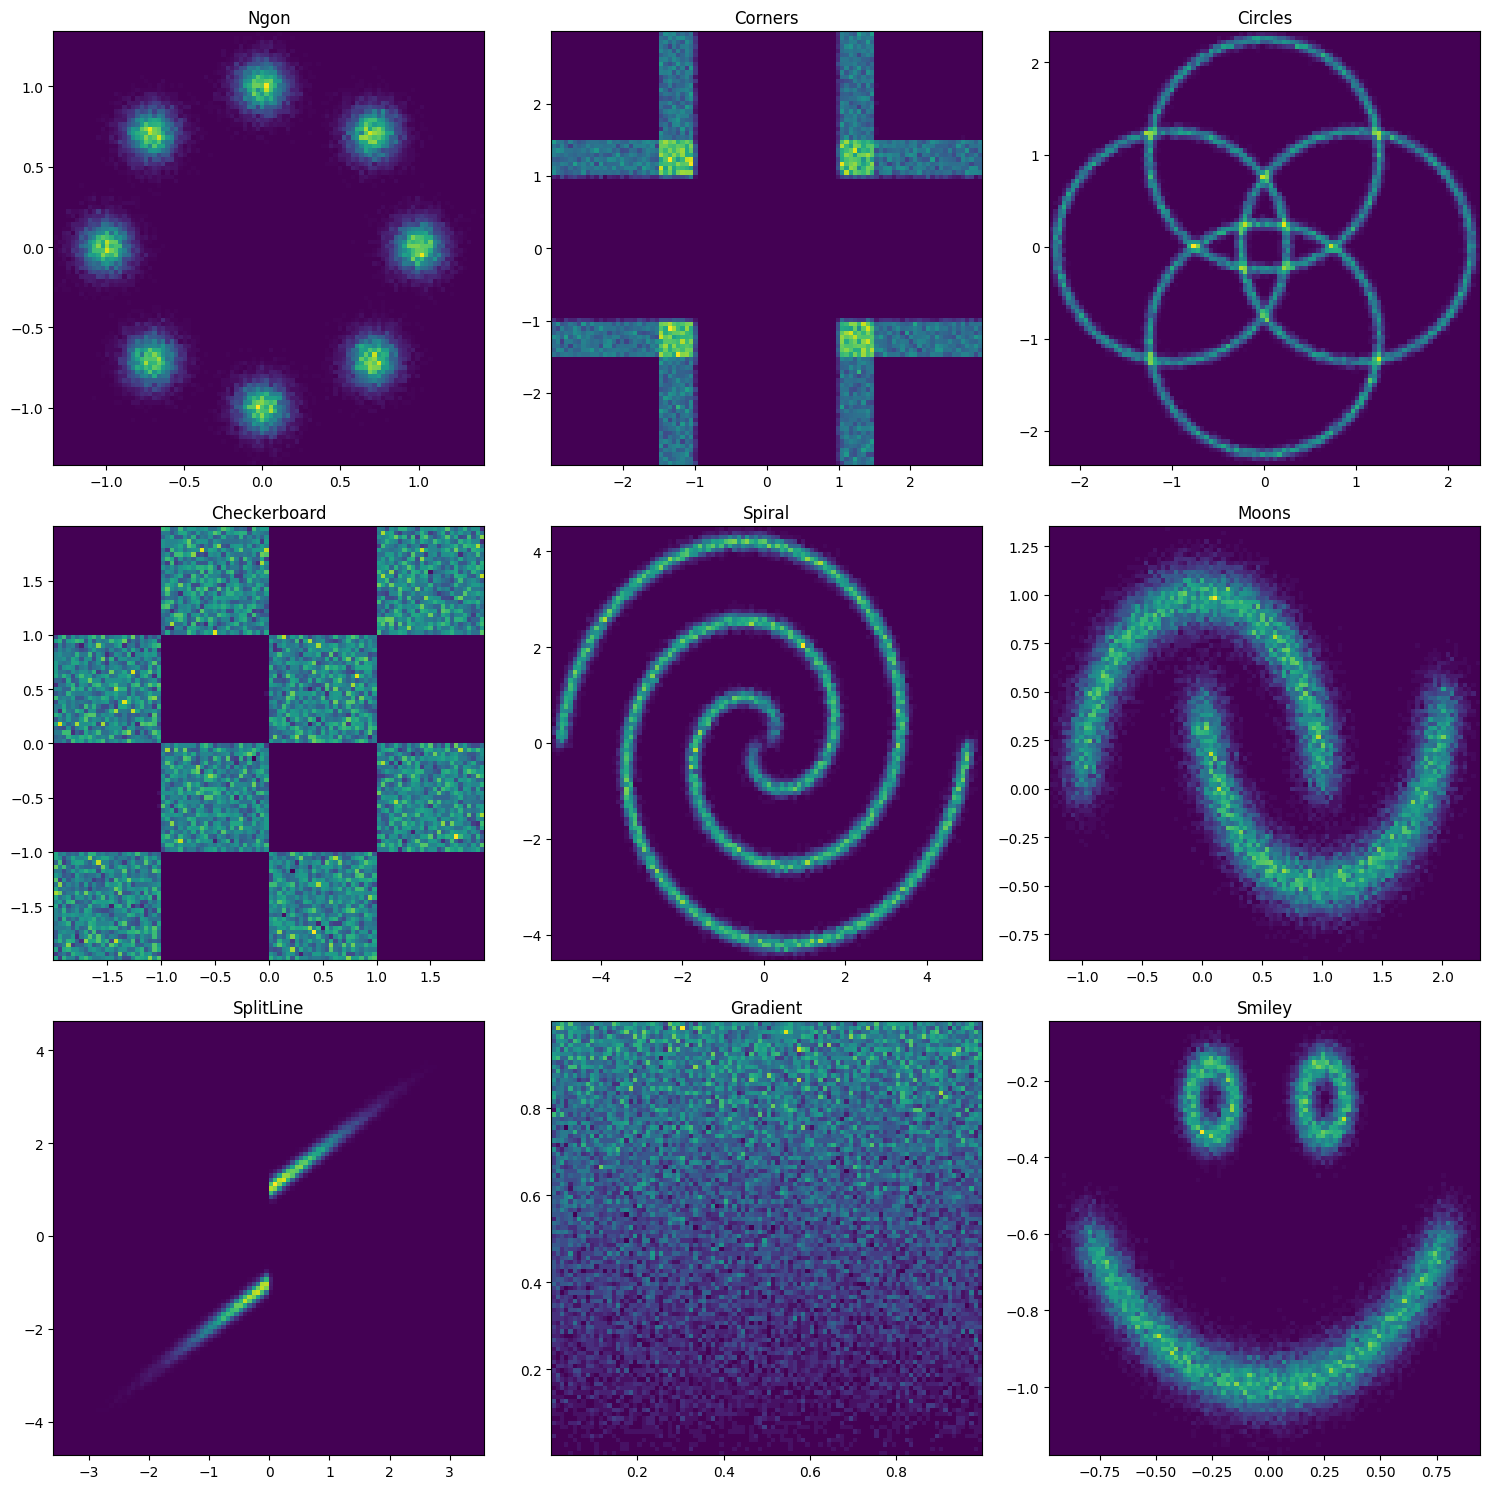
\includegraphics[width=\textwidth]{images/synthetic/overview/synt-nolab.png}
\caption{Synthetic unlabeled datasets ($10\,000$ samples each).}\label{fig:synt-nolab}}

\vspace{2em}

\dataset{Ngon} $n$ Gaussians with constant noise arranged along a circle.

\dataset{Corners} $4$ disjoint corners with overlaps (with doubled density).

\dataset{Circles} $n$ circles with equal radius arranged along a circle.

\dataset{Checkedboard} a tiling of size $n^2$, sampling only one tile color.

\dataset{Spiral} a double spiral, symmetric around the origin.

\dataset{Moons} the standard two moons dataset.

\dataset{SplitLine} A thin Gaussian separated by an offset in the middle.

\dataset{Gradient} Essentially noise -- randomly sample $x$, $x^2$ and concatenate.

\dataset{Smiley} a combination of two circles and a semi-circle.
\end{figure}

\begin{figure}
\centering
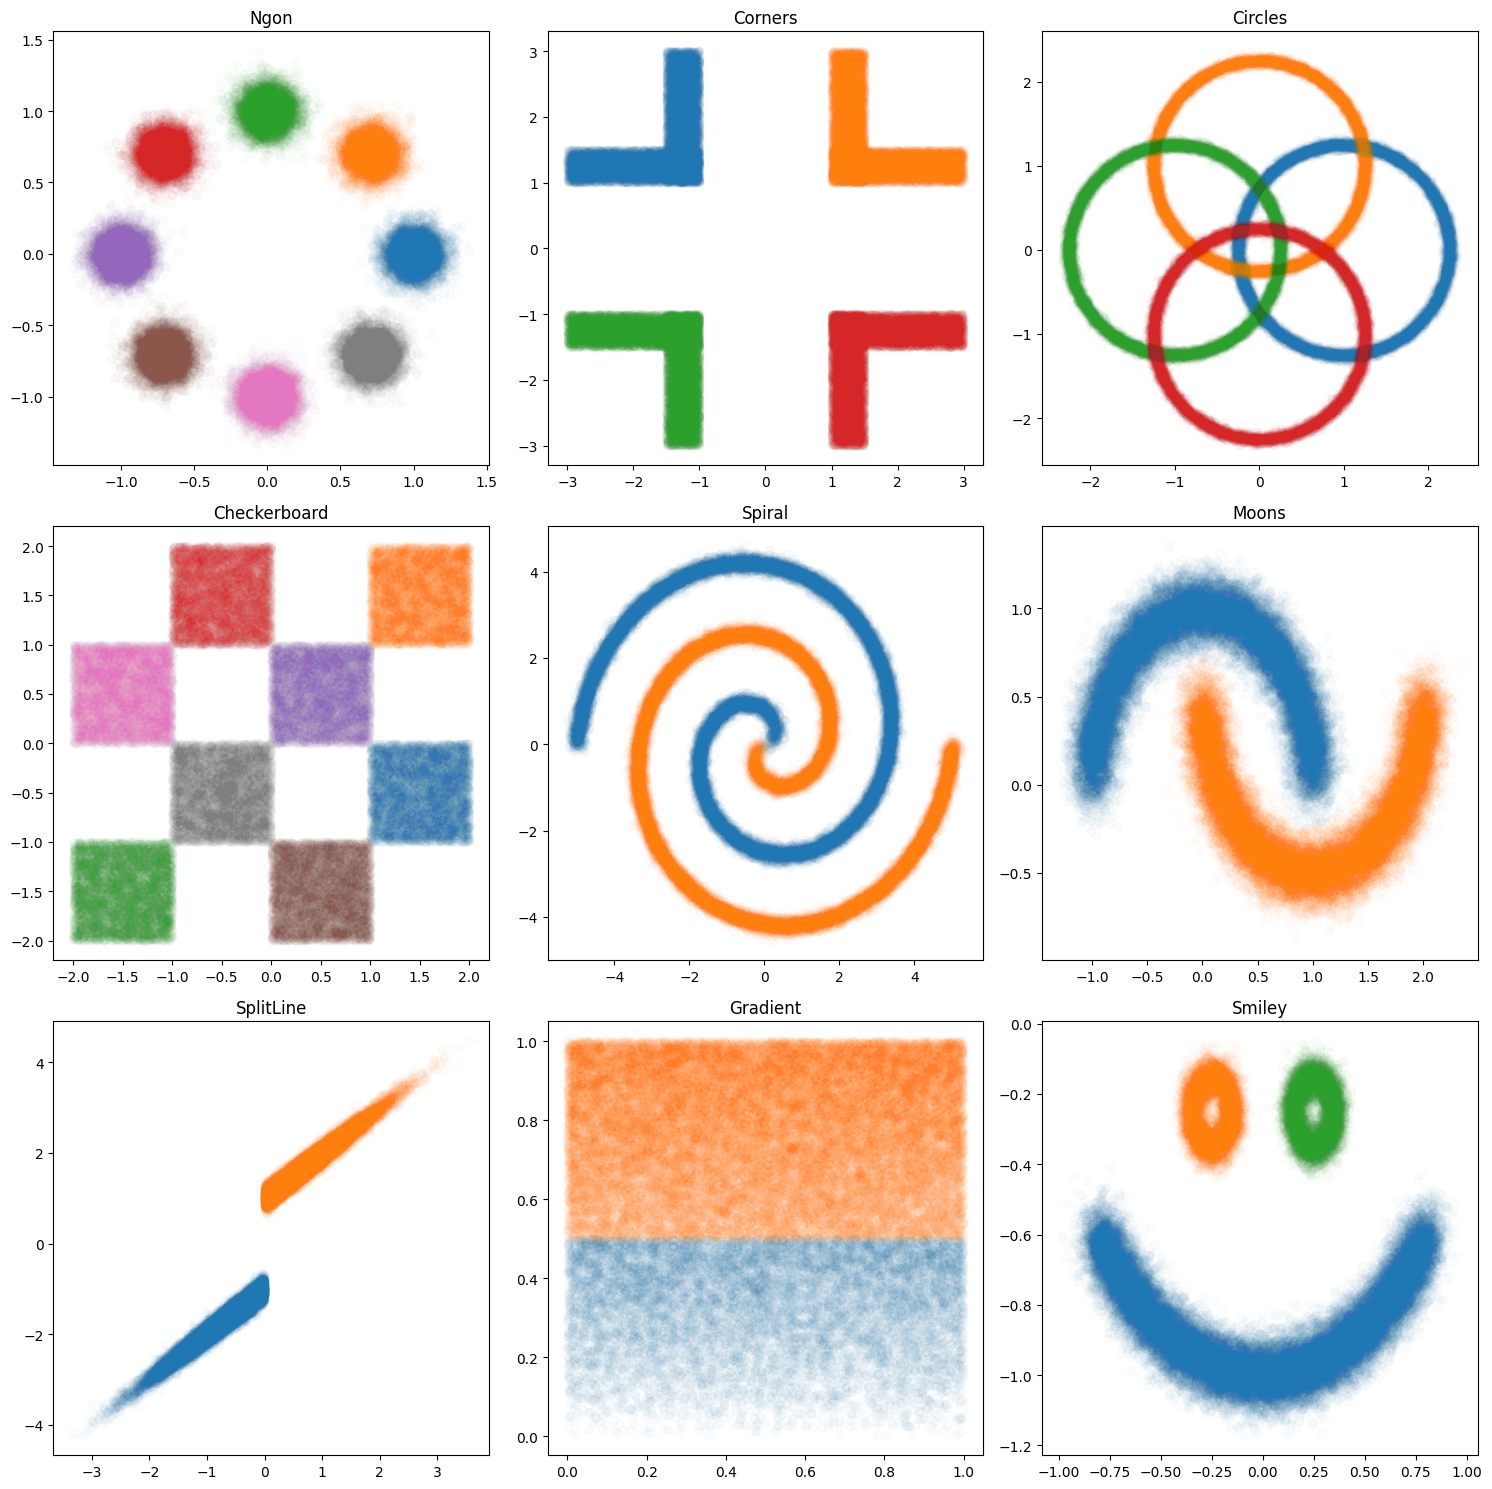
\includegraphics[width=\textwidth]{images/synthetic/overview/synt-lab.png}
\caption{Synthetic labeled datasets ($10\,000$ samples each). The categories were picked in the most intuitive way, also making sure that each dataset has $ \geq 2$.}\label{fig:synt-lab}
\end{figure}

\begin{figure}
\centering
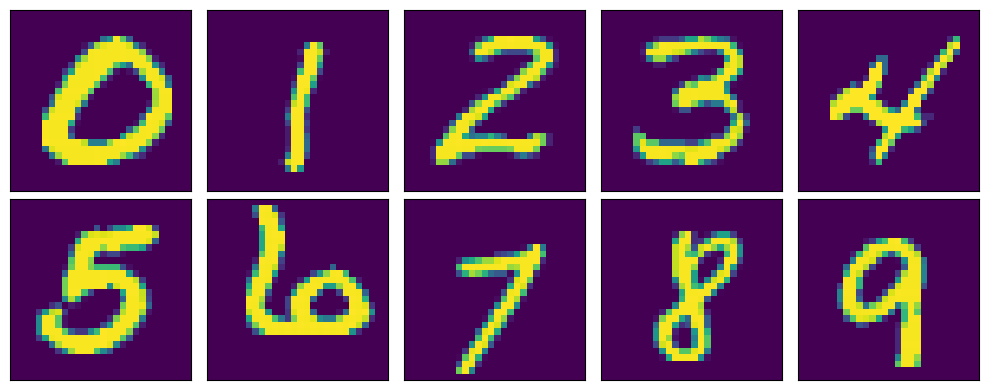
\includegraphics[width=\textwidth]{images/mnist_maxpooling/mnist_dataset.png}
\caption{Example images from the MNIST784 dataset.}
\label{fig:mnist784_example}
\end{figure}


\asubsubsection{Image Data}{Jannis Heising}
As reasoned in Section~\ref{sec:image_data}, we used the MNIST784 dataset for our image data experiments as opposed to the more complex sets used in~\cite{nielsen2020survae}. MNIST784 consists of 70,000 grey-scale images, each of size 28x28 and displaying one of the ten digits 0-9, as shown in Figure~\ref{fig:mnist784_example}.


\asubsubsection{Point Cloud Data}{Maria Stickel}

Similar to \cite{nielsen2020survae} and \cite{edwards2017neural}, we wanted to train our model on the spatial MNIST data set, where instead of directly using the images of hand-written digits, one uses the probability weights over the images of the hand-written digits to sample coordinates for single points which together as a cloud represent the digit.

In general, one input vector to the network describes a single point sampled from the underlying distribution. In the synthetic datasets, this is a single point from a two-dimensional vector space, drawn from the underlying distribution. In the case of the point cloud data, a single input point is a cloud of points and therefore contains several point samples from the distribution of weights over the image. This resulted in quite some issues when applying the previously easy-to-use modular framework of layers, where we saw very good results pretty fast.

Our initial approach on how to handle the points was pretty much "flatten everything" and "unflatten if necessary". An example of this is be the \texttt{MaxPoolingLayer} (\ref{sec:max_pooling_layer}) operation for the previously described plain MNIST dataset. For the spatial MNIST data, operations like permutations break the structure of the array in the sense as it would not permute the sampled points as tuples, but also permute points and their x- and y-coordinates, removing the possibility for the model to understand the underlying dependencies of the coordinates. Therefore we introduced layers that don't appear in \cite{nielsen2020survae}: \texttt{PermuteAxesLayer} (\ref{sec:permute_axes_layer}) and \texttt{ReshapeLayer} (\ref{sec:reshape_layer}) to address this issue. We also modified the \texttt{BijectiveLayer} to operate on this type of structured data, which was a changing point for the results (see \ref{sec:spatial_mnist}).

Both referenced papers used 50 points to represent a digit, and in our final experiments we followed their approach. Initially, we also experimented with a smaller number of points, 30 to be exact, as we were curious to see whether this is sufficient, but the results were worse. We dropped that and don't include it here. 

\asubsubsection{SIR Data}{Jannis Heising}\label{sec:sir_data}
The SIR model aims to describe how an infectious disease spreads throughout a population. The population $N$ is spread into three \textit{compartments}, namely Susceptible $S$, Infectious $I$, and Removed $R$. For simplicity, the population size is normalized to 1, meaning that the values $S$, $I$, and $R$ represent the \textit{fraction} of the population belonging to that compartment.

Given these fractions, the SIR model prescribes their rate of change as an ordinary differential equation (ODE):
\begin{align*}
    \frac{\dd S}{\dd t} &= -\lambda \cdot S \cdot I,\\
    \frac{\dd I}{\dd t} &= \lambda \cdot S \cdot I - \mu \cdot I,\\
    \frac{\dd R}{\dd t} &= \mu \cdot I.
\end{align*}

Here, $\lambda$ and $\mu$ are parameters that determine the behaviour of the system. The other parameters are the \textit{initial values} $S_0$, $I_0$, and $R_0$ of the fractions at time {$t = 0$}. To simplify the model, we always set {$S_0 = R_0 = 0$}. Thus, the system behaviour is completely determined by the three parameters $\lambda$, $\mu$, and $I_0$.

In the setting of SBI, these three values are the \textit{hidden parameters}. A simulation then produces their corresponding \textit{observational data}. We use a simple Euler-forward method with step size 0.1 to simulate the ODE above for 100 days (i.e. until {$t = 100$}). The data then consists of the rate-of-change values $\frac{\dd S}{\dd t}$ and $\frac{\dd R}{\dd t}$ at each step.

\asubsection{Parameter Degeneracy and SBI}{Jannis Heising}\label{sec:background_param_degen}

One of our experiments revolves around parameter degeneracy of simulation-based inference (SBI), thus we briefly introduce those terms.

\textbf{Simulation-based Inference (SBI)} is a method for identifying hidden parameters of observational data with the help of an existing simulation. A prime example is understanding the spread of a disease when given infection rate data on one hand and a theoretical framework in the form of a simulation on the other. The simulation takes the hidden parameters and turns them into observation-like data, so SBI can be thought of as an inverse to the simulation.

In practical terms, the setup for SBI is as follows: Let $\{Y_k^{*}\}_{k=1}^K$ be $K$ sets of hidden parameters and $\{X_k = \Phi(Y_k^{*})\}_{k=1}^K$ their respective outputs of the simulation $\Phi$. We then train a conditional NF on the dataset $\{(Y_k; X_k)\}_{k=1}^K$, i.e. we train it to generate the parameters $Y_k$ given the condition $X_k$.

\textbf{Parameter degeneracy}, in the context of this report, is a shortcoming of normalizing flows which occurs when the data manifold does not have the same dimension as the latent space. For example, if one were to train a two-dimensional NF on points lying solely on a one-dimensional shape like a circle embedded in two-dimensional euclidean space, one would be presented with an underwhelming result (see Section~\ref{sec:simple_degen}).

In the lecture, we briefly touched on parameter degeneracy in the context of SBI: It may happen that not all hidden parameters can be unequivocally recovered from the observed data. As an example, we chose the most basic SIR model (see Section~\ref{sec:sir_data}). Note that the article uses $\beta$ and $\gamma$ instead of $\mu$ and $\lambda$. with only three parameters $\mu$, $\lambda$, and $I_0$ and made it degenerate by replacing $\lambda$ with two new parameters $\lambda_1$ and $\lambda_2$. For the simulation, these values are multiplied to end up with only one value $\lambda = \lambda_1 \cdot \lambda_2$, thus the original two values cannot be recovered from the simulation output alone.

\section{Methods}\label{sec:methods}

\asubsection{Layers}{Maria Stickel}\label{sec:layers}

In the following we'll describe the different layers we implemented. We define $\mathcal{LL}$(\texttt{Layer}) to be the log-likelihood contribution of \texttt{Layer}. We refrain from deducing the formulas for bound looseness and likelihood contribution and refer the reader to \cite{nielsen2020survae}.

All of the layers are defined in the inference direction, i.e. the `forward' method sends elements of the data space $\mathcal{X}$ to the latent space $\mathcal{Z}$, whereas the `backward' method goes from $\mathcal{Z}$ to $\mathcal{X}$.

The layers can be separated in two groups: stochastic and non-stochastic\footnote{In \cite{nielsen2020survae} they refer to the non-stochastic layers as bijective. This was a little confusing in the beginning as some stochastic layers are (in theory) bijective operations on the data (permutations) but also stochastic in the sense that they operate differently in different execution calls on the \textbf{same} data.}. The forward call implements the mapping $\mathcal{X} \rightarrow \mathcal{Z}$. All of our layers are vectorized over the batch size. 


\asubsubsection{\texttt{BijectiveLayer}}{Maria Stickel}\label{sec:bijective}
Standard bijective transformation from normalizing flow architecture. In the forward pass, the input vector is divided into two parts: On the skip part no transformations are applied, but the input is simply passed on as it is. Yet, it serves for the calculation of the bijective non-identity transformation applied to the other part of the data.

Firstly, the skipped input is fed to a standard feed-forward neural network which generates the coefficients $(s,t)$ of the linear transformation applied to the non-skip part. The backward pass (or generative direction) is the inverse transformation. The likelihood contribution of a bijective (non-stochastic) transformation is $ \log | \det (J)|$ where $J$ is the Jacobian of the transformation which in the case of our chosen linear transformation \eqref{eq:bijective} results in a log-likelihood contribution of \eqref{eq:ll_bijective}. 
\begin{equation}
\texttt{ BijectiveLayer} (X_i) = \left\{ \begin{array}{rl}X_i & \text{for $i$ in skip connection} \\ e^{\tanh(s_i)} \cdot X_i + t_i & \text{for $i$ in non-skip connection} \end{array} \right.
\label{eq:bijective}
\end{equation}
\begin{equation}
    \mathcal{LL}\texttt{(BijectiveLayer)}= \sum_{i} \tanh(s_i)
    \label{eq:ll_bijective}
\end{equation}
In the case of labelled input, the bijective layer applies the same transformation, except for the skip-connection, that is extended by the labels. We had quite some issues with this layer in the context of the Point Cloud data described in section \ref{sec:spatial_mnist}. The first version of the layer was structured in a way that it accepted a flattened input vector representing one "point of data" and applied its transformation to it. So we modified it to accept tuples of shape, that we flatten (in the final version of the implementation). The purpose and functionality of the layer is the same as before. The layer applies the bijective transformation to the last \texttt{skip\textunderscore size} points in the point cloud.

\asubsubsection{\texttt{OrthonormalLayer}}{Maria Stickel}\label{sec:orthonormal}
Applies orthonormal transformation and its inverse. Unlike other layers, the transformation is randomly sampled upon initialization and applied every time the network is called (i.e. no training). The likelihood contribution is obviously zero as the determinant of the Jacobian of an orthonormal transformation is one. It is obviously a bijective module. In the case of spatial MNIST, we used a more specific version of this layer (transposition layer), which we did not implement as a separate layer, which swaps the x- and y-components.

\asubsubsection{\texttt{MaxTheLayer}}{Maria Stickel}
The forward pass consists of taking the maximum over the entire input, while the backward pass samples an index $k$ for the maximum value based on a categorical distribution (whose weights can be learned in training) and subtracts values sampled from the half-normal distribution from the maximum value in all other entries. Its variance $\sigma$ can and should be learned and is initially set to $0.1$. The layer is clearly stochastic and therefore has a non-trivial contribution to the log-likelihood approximated in the following way\footnote{A deduction of this can be found in \cite{nielsen2020survae}, more specifically in Appendix E.}.
\begin{equation}
\mathcal{LL}(\texttt{MaxTheLayer}) \approx
   \sum_{i = k} \log p(\text{i}|Z) + \sum_{i \neq k} \log q(X_i|Z,k) 
\end{equation}

\asubsubsection{\texttt{MaxPoolingLayer} \& \texttt{MaxPoolingLayerWithOverlap}}{Maria Stickel}\label{sec:max_pooling_layer}
We implemented a surjective layer with stochastic backward pass that reduces 2-dimensional input data by taking the local maximum over blocks of it. Note that, as mentioned above, the input is generally flattened, so the layer un-flattens the given input\footnote{Which requires flattened-data-shape to be a square nummber.} and then performs the MaxPooling operation. The \texttt{MaxPoolingLayer} has no overlap between blocks, any entry is used for calculation of exactly one local maximum, equal to the layer in \cite{nielsen2020survae}.

In the generative direction of \texttt{MaxPoolingLayer} (the backward pass), the maximum is arbitrarily assigned to one position in the corresponding block and all other block entries are sampled as smaller values by subtracting values sampled by a half-normal (default) or an exponential distribution (choice upon layer definition) from the block maximum (see Table~\ref{table:maxpool_distributions}). Therefore, the log-likelihood contribution is essentially the same as that of \texttt{MaxTheLayer}, just repeated for each block. Distribution parameters are parameters that can be trained (design choice). We recommend to use the option to train them. At this point it is worth mentioning that one could have further extended the flexibility of the layer by training a classifier to assign the argmax value in a block. Another reasonable extension of functionality would be to use several distributions for sampling the values-to-be-subtracted for the \texttt{MaxPoolingLayer}, with different possible parameters i.e. one per block, or one per several blocks, to further adapt to the distribution of the underlying data. These different granularities are a hyperparameter, which we chose to set to one, considering the scope of the project.
\begin{table}[H]
    \centering
    \begin{tabular}{lcc}
    \toprule
    & Half-Normal & Exponential \\
    \midrule
    Formula & $f(x; \sigma) = \sqrt{\frac{2}{\pi}} \frac{1}{\sigma} e^{-\frac{x^2}{2\sigma^2}}$ & $f(x; \lambda) = \lambda e^{-\lambda x}$ \\
    Parameters & $\sigma > 0$ & $\lambda > 0$ \\
    \bottomrule
    \end{tabular}
    \caption{The two distributions that we implemented for \texttt{MaxPoolingLayer} and \texttt{MaxPoolingLayerWithOverlap}.}
    \label{table:maxpool_distributions}
\end{table}
We extended the functionalities in \cite{nielsen2020survae} by implementing a \texttt{MaxPoolingLayerWithOverlap} which is similar, but allows for overlap between the blocks over which the maximum is taken. Figure \ref{fig:both_maxpoolings} illustrates \texttt{MaxPoolingLayerWithOverlap} for different hop sizes, where the stride indicates the block size, the hop is the offset from one block to the next and the width is the width of the picture/data. Strictly speaking, \texttt{MaxPoolingLayer} is a special case of \texttt{MaxPoolingLayerWithOverlap} with stride=hop. For simplicity all input data is assumed to be square.
\begin{figure}
    \centering
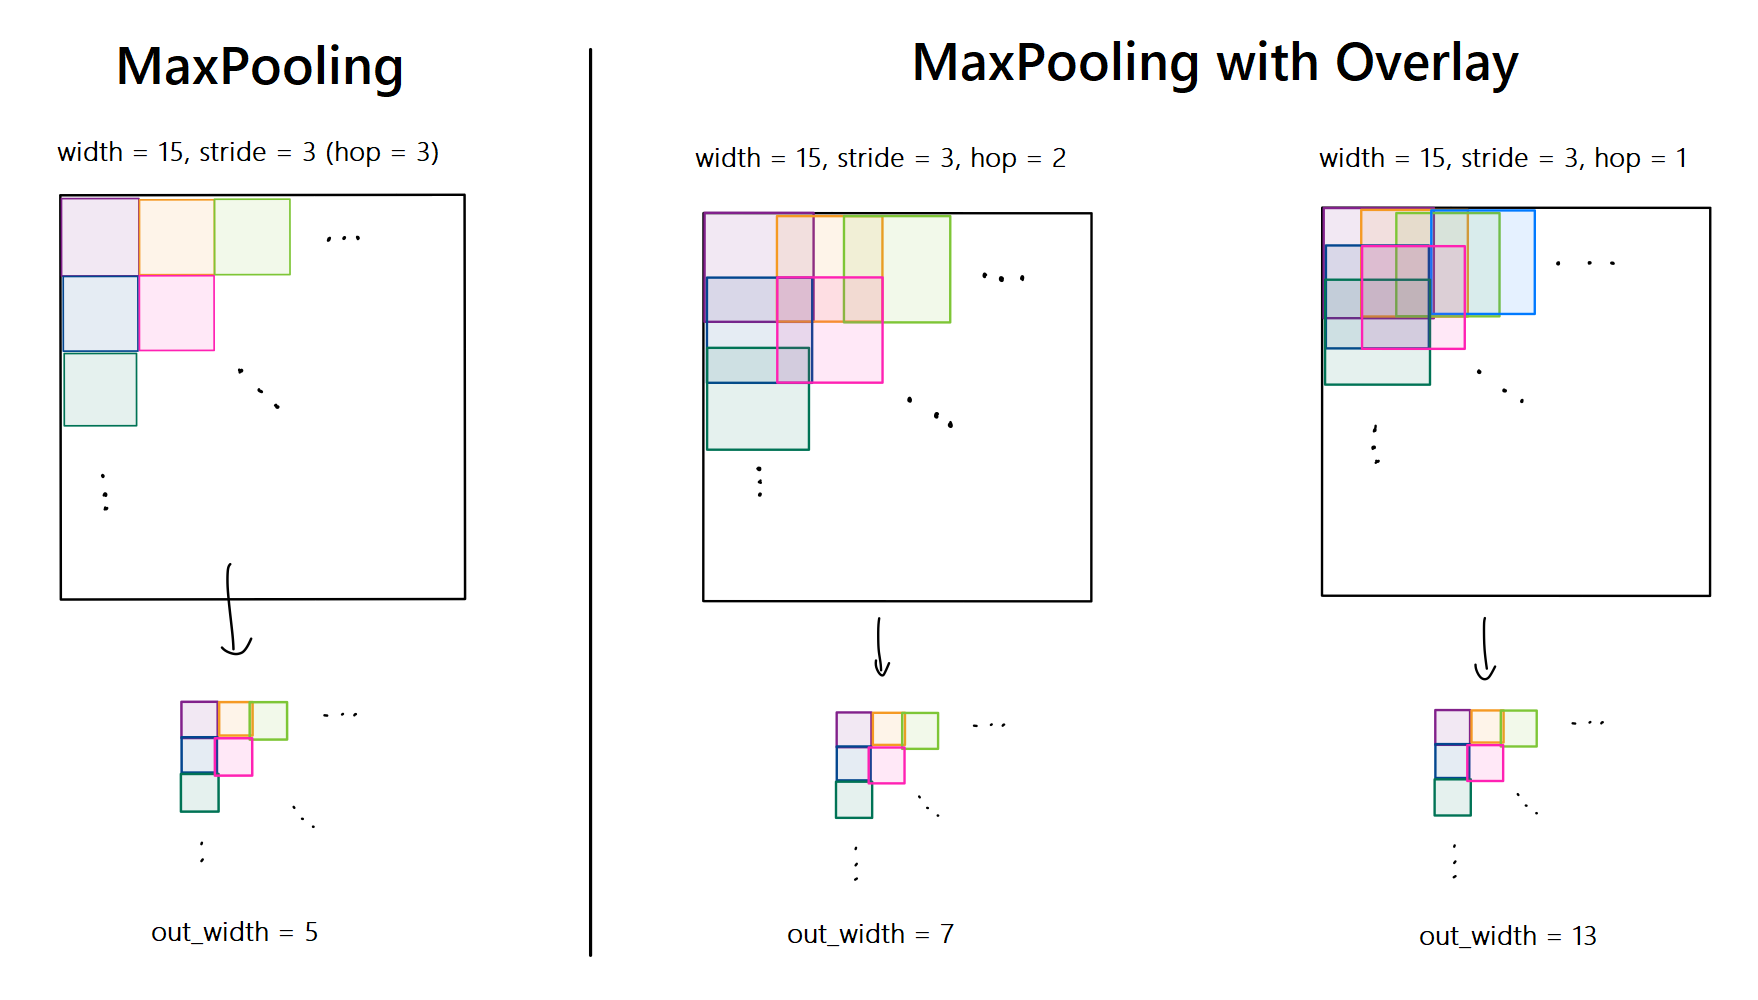
\includegraphics[width=\textwidth]{images/layers/BothMaxPoolings.png}
    \caption{Different parameters for \texttt{MaxPoolingLayerWithOverlap}. The smaller the hop, the larger the output size.}\label{fig:both_maxpoolings}
\end{figure}

The backward pass of \texttt{MaxPoolingLayerWithOverlap} requires a different approach, as the overlap between blocks poses several constraints on an entry, as it needs to be smaller or equal to the smallest maximum of all blocks containing it. We calculate the smallest such maximum for each entry and then sample an index for our maximum in the fields where it actually can be assumed (data-dependent), while subtracting values sampled from a half-normal or an exponential distribution (design choice) with learned parameters.

Similarly to the version of the layer without the overlap, one could think about learning several half-normal or exponential distributions for values to be subtracted. Yet, using a classifier to sample a random index to place the maximum proves to be much more difficult, as candidate amount and location changes depending on the data. We constrained our use cases to square 2D data and used square blocks, but more complex data and block shapes could be used. The approximation of the log-likelihood is similar to the one in \texttt{MaxTheLayer}, only that it's a little bit more complex in practice to perform the computation for all the different blocks.

\asubsubsection{\texttt{SortingLayer}}{Maria Stickel}\label{sec:sorting_layer}
In the forward pass, this layer performs a sorting operation along the last axis. Use cases can be naturally sorted data, exchangeable models and order statistics. It is a stochastic surjective transformation, as we cannot recover the original order of the vector. The backward pass is a random permutation.

We implemented a helper function both for \texttt{SortingLayer} and \texttt{PermutationLayer}, to enable a vectorized treatment of the batch. It applies a random permutation to the last axis of X for each entry along its first axis, and is used in the backward pass of the Sorting Layer. There is a possibility to replace the random permutation in the backwards pass with a categorical distribution with learned parameters, which we did not pursue, making the log-likelihood of this operation zero.


\asubsubsection{\texttt{PermutationLayer}}{Maria Stickel}\label{sec:permutation_layer}
This layer randomly shuffles in both the inference and the generative direction, with a new permutation in each call. This is a stochastic operation with zero contribution to the log-likelihood. Is is used in each block for the Point Cloud data (section \ref{sec:spatial_mnist}) to enforce permutation invariance. 


\asubsubsection{\texttt{AbsoluteLayer}}{Maria Stickel}\label{sec:absolute_layer}
This layer performs the absolute value inference surjection. The forward pass is simply taking the absolute value of each entry abs$(X)$. In the backward pass, we sample signs $S$ for all the values in $Z$, using a parameter $q$ (which can be trained or set to a fixed value like $\frac{1}{2}$), which is the event probability of sampling a positive sign, and then return the product of the signs with the data $\hat{X} = S \cdot Z$. The log-likelihood contribution is described in \eqref{eq:ll_absolute} and corresponds to the log-likelihood contribution derived in \cite{nielsen2020survae}, except for the fact that they describe it for one-dimensional input while we extend it to higher-dimensional input (summation). 
\begin{equation}
\mathcal{LL}\text{(\texttt{AbsoluteLayer})} = \#\{S_i : S_i = 1\} \cdot \log(q) +  \#\{S_i : S_i = -1\} \cdot \log(1 - q)  \label{eq:ll_absolute}
\end{equation}
We experimented with different values for $q$, which in theory is supposed to be in $[0,1]$. As it is a trained parameter, it can escape those reasonable bounds. Read more about this in section \ref{sec:exp_and_results}.


\asubsubsection{\texttt{DequantizationLayer}}{Maria Stickel}\label{sec:dequantization_layer}
This layer's purpose is to un-discretize, which is adding random noise in $(0,1)$ in the forward pass to quantized input data\footnote{Or in programming terms: convert from integer to double (or float).}. This is necessary as we want to be able to generate discrete data while sampling from a Gaussian, which requires de-quantization in the forward pass. The backward pass is a rounding operation (floor). The log-likelihood of this operation is zero as we use a uniform distribution over the noise interval. We used it for image data, see section \ref{sec:image_data}.


\asubsubsection{\texttt{AugmentLayer}}{Maria Stickel}
As the name suggests, we augment input data by extending data points with randomly sampled values in the forward pass and removing them in the backward pass. In our implementation, we don't learn distribution parameters, but only sample from a standard normal distribution. Therefore in our case the log-likelihood contribution is zero. If given more time, we could have implemented different distributions with their respective (trainable) parameters. The layer has proven to be useful in datasets based on discontiguous distributions (e.g. the two moons dataset). It is surjective in the generative direction.


\asubsubsection{\texttt{SliceLayer}}{Maria Stickel}
This layer is the opposite of \texttt{AugmentLayer}. In the forward pass, we remove elements from the input vector and in the backward pass we augment it. The log-likelihood contribution is zero for the same reason.

\asubsubsection{\texttt{PermuteAxesLayer}}{Maria Stickel}\label{sec:permute_axes_layer}
As the name suggests, this layer permutes the axes of the vector space. Obviously, this is only useful for multi-dimensional data and is used in particular for the Point Cloud Data.


\asubsubsection{\texttt{ReshapeLayer}}{Maria Stickel}\label{sec:reshape_layer}
A layer to reshape data vectors. We implemented it for the spatial MNIST dataset, to reshape the output to point cloud elements.

\asubsection{Training}{Tomáš Sláma}

The training of all models was done via the Adam optimizer in batches of size $k$, meaning each of the $n$ epochs sampled $k$ values $X$ from the dataset function.
It then ran $X$ forward through the network, obtaining the values in latent space $Z$, along with the log-likelihood $\mathcal{LL}$, and ran a step of the optimizer on their sum; more specifically: $$\mathcal{L}\text{oss} = 0.5 |Z|^2 - \mathcal{LL}$$
The training also supports decaying the learning rate (which was used for most of the examples) and providing the layers with conditional vector, which was used for training conditional networks (by influencing how the log-likelihood was calculated).

Besides returning the trained network, the training function also saved state snapshots and losses on an evaluation set to prevent overfitting in an orderly way, making plotting easy. 

\asubsection{Model Evaluation}{Jannis Heising}

Since the two-dimensional synthetic distributions (Section~\ref{sec:synthetic}) are easy to visualize, our main evaluation tool was our own judgment of the distribution plots. Additionally, we always plotted the training and validation losses. Where appropriate, we sought to visualize the behaviour of the novel models from~\cite{nielsen2020survae} in the form of ``Q-plots" (Figure~\ref{fig:skewed-q}) and symmetry axes (Figure~\ref{fig:symmetries_checkerboard}) for the \texttt{AbsoluteLayer}.

For the higher-dimensional datasets, we visualized the code distribution of the trained models by taking the output {$Z = f(X)$} of a model $f$ from a data sample $X$ and plotted one-dimensional and two-dimensional slices of $Z$ (see for example Figure~\ref{fig:spatial_mnist_code_after}). The 1D slices are overlaid with the probability density function of the standard Normal distribution $\mathcal{N}(0, 1)$ and the 2D slices show its 90\% confidence interval for an intuitive visual cue of how well the distributions match (both in red).

Additionally, we used calibration diagrams to gauge how well the samples from a given model fit the observed data distribution (see Figure~\ref{fig:sir_run_1}). Without going into detail, a calibration diagram shows in which ``parts" of the data distribution a given sample (or set of samples) is likely to fall. Ideally, all bars have the same height, indicated by a red dotted line. We ended up only using this tool for the SBI data (Section~\ref{sec:sbi}) because it is fairly low-dimensional but could have theoretically used it for all other tests as well.

The SBI models additionally provided the option to use resimulation diagrams (see Figure~\ref{fig:sir_run_2}): Given an initial set of parameters $X$, one takes the corresponding simulation data $Y$ and generates samples {$\hat{X} = f^{-1}(Z|Y)$} from a trained model $f$. These samples are fed to the simulation to obtain simulation data $\hat{Y}$. One can then determine whether the original data $Y$ lies within the 90\% confidence interval of the new data $\hat{Y}$ by plotting them together.

While trying to find the error in the \texttt{BijectiveLayer} log-likelihood contribution described in Section~\ref{sec:image_data}, we additionally started logging the standard deviation of the code distribution. It turned out that it behaved very similarly to the loss (see Figure~\ref{fig:mnist_run_4_loss_vs_sigma}), so we chose not to mention it except here.

\begin{figure}
\centering
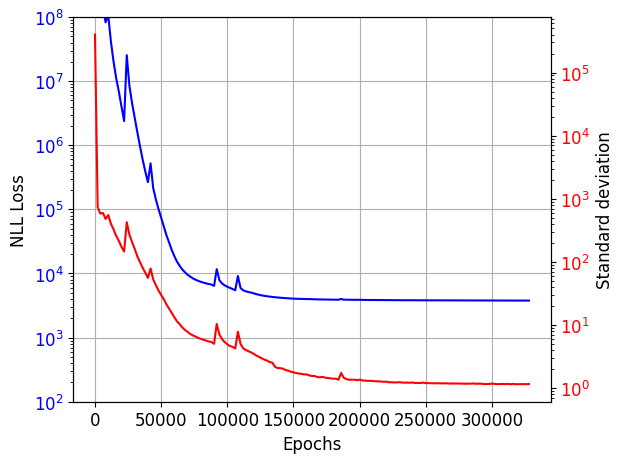
\includegraphics[width=.7\textwidth]{images/mnist_maxpooling/run_4_loss_vs_sigma.png}
\caption{Validation loss and standard deviation from Experiment 4 on the MNIST784 dataset.}
\label{fig:mnist_run_4_loss_vs_sigma}
\end{figure}
\section{Experiments and Results}\label{sec:exp_and_results}

\subsection{Synthetic Data}\label{sec:synthetic}

\asubsubsection{\texttt{AbsoluteLayer} -- Unlabeled}{Tomáš Sláma}

\textit{The results are taken from the \href{https://github.com/xiaoxiae/GNNFinal2024/blob/main/notebooks/abs.ipynb}{notebooks/abs.ipynb} notebook.}

The initial experiment was to compare performance on the four datasets the original paper used with the following baseline network architecture (NF). The sizes of the layers were chosen to sufficiently capture the complexity of all of the datasets:


\begin{minted}{python}
(BijectiveLayer(2, [64] * 5), OrthonormalLayer(2)) x 10
\end{minted}

To utilize the symmetry of the data, this architecture was compared with one that has an absolute layer at the beginning (NF-abs):

\begin{minted}{python}
AbsoluteLayer(2)
(BijectiveLayer(2, [64] * 5), OrthonormalLayer(2)) x 10
\end{minted}

The results can be seen in figure \ref{fig:abs-default}. Unless specified otherwise, all networks in this section were trained for $1\,000$ epochs with a learning rate $0.001$ and batch size $1\,000$.

\begin{figure}[H]
    \centering
    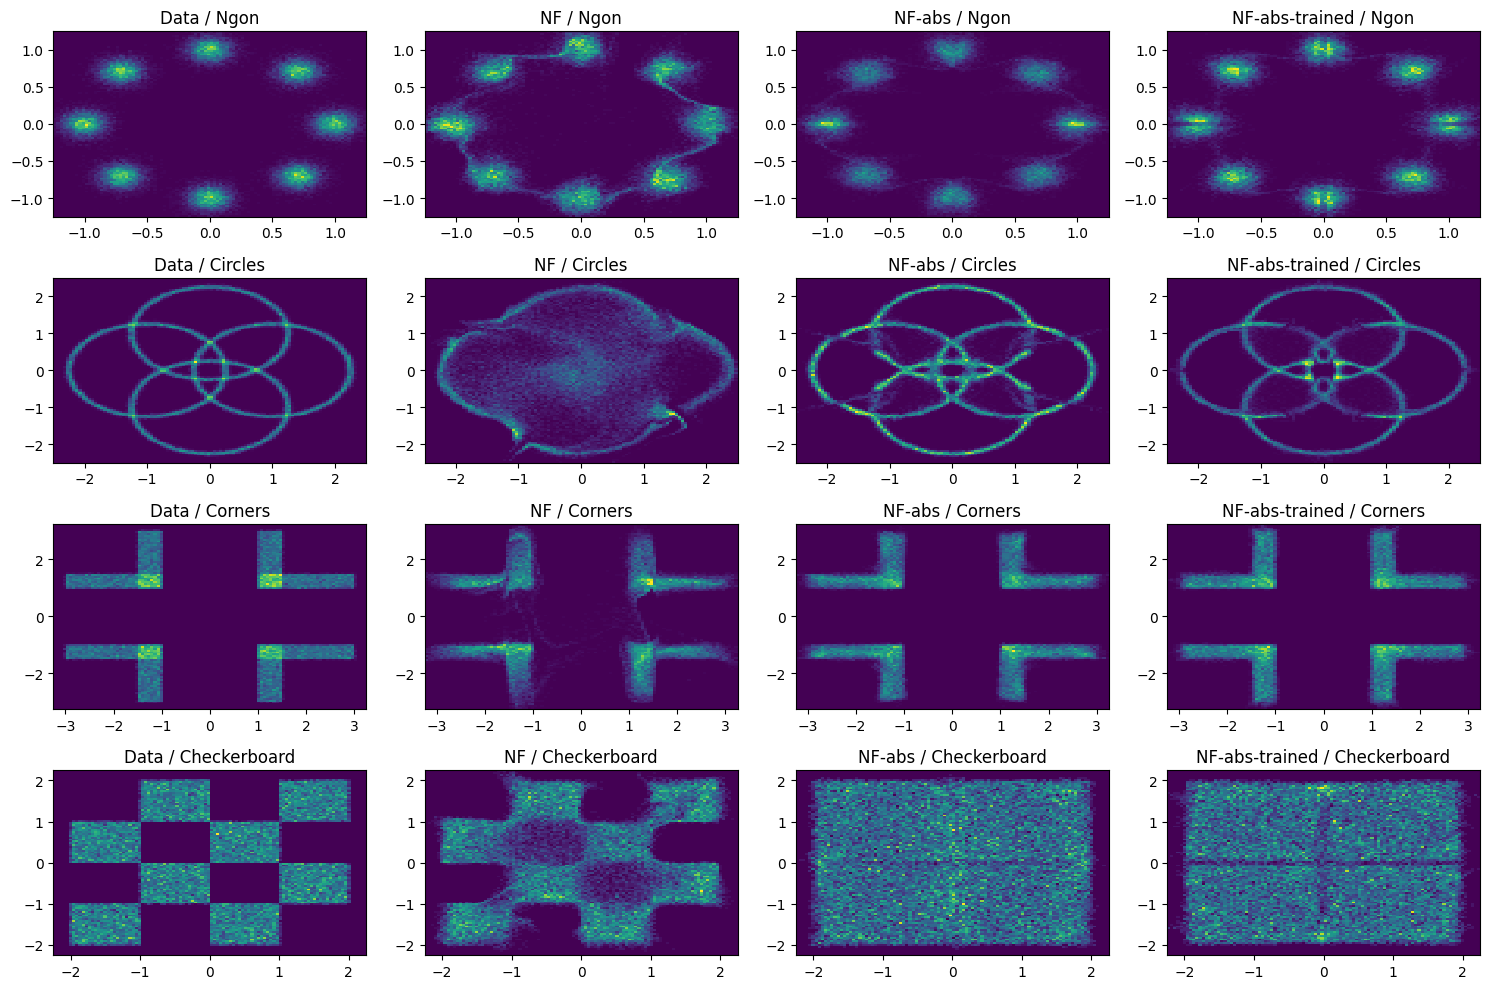
\includegraphics[width=.85\linewidth]{images/synthetic/abs-default.png}
    \caption{Comparison of methods for synthetic datasets; ground truth (column 1), baseline network architecture (column 2), architecture with absolute layer at the beginning with a fixed Q-tensor (column 3) and architecture with absolute layer at the beginning with a learned Q-tensor (column 4).}
    \label{fig:abs-default}
\end{figure}

As we see, the architectures with the absolute layer (columns 3 and 4) perform much better, which is no surprise since it dictates the symmetry in both axes and is therefore much easier to train.

As a sanity check, the models were also trained on skewed data (i.e. $50\%$ of values were randomly flipped about the Y-axis) to see if the absolute layer learned the correct Q-tensor. The result can be seen in Figure \ref{fig:abs-skewed}.

\begin{figure}[H]
    \centering
    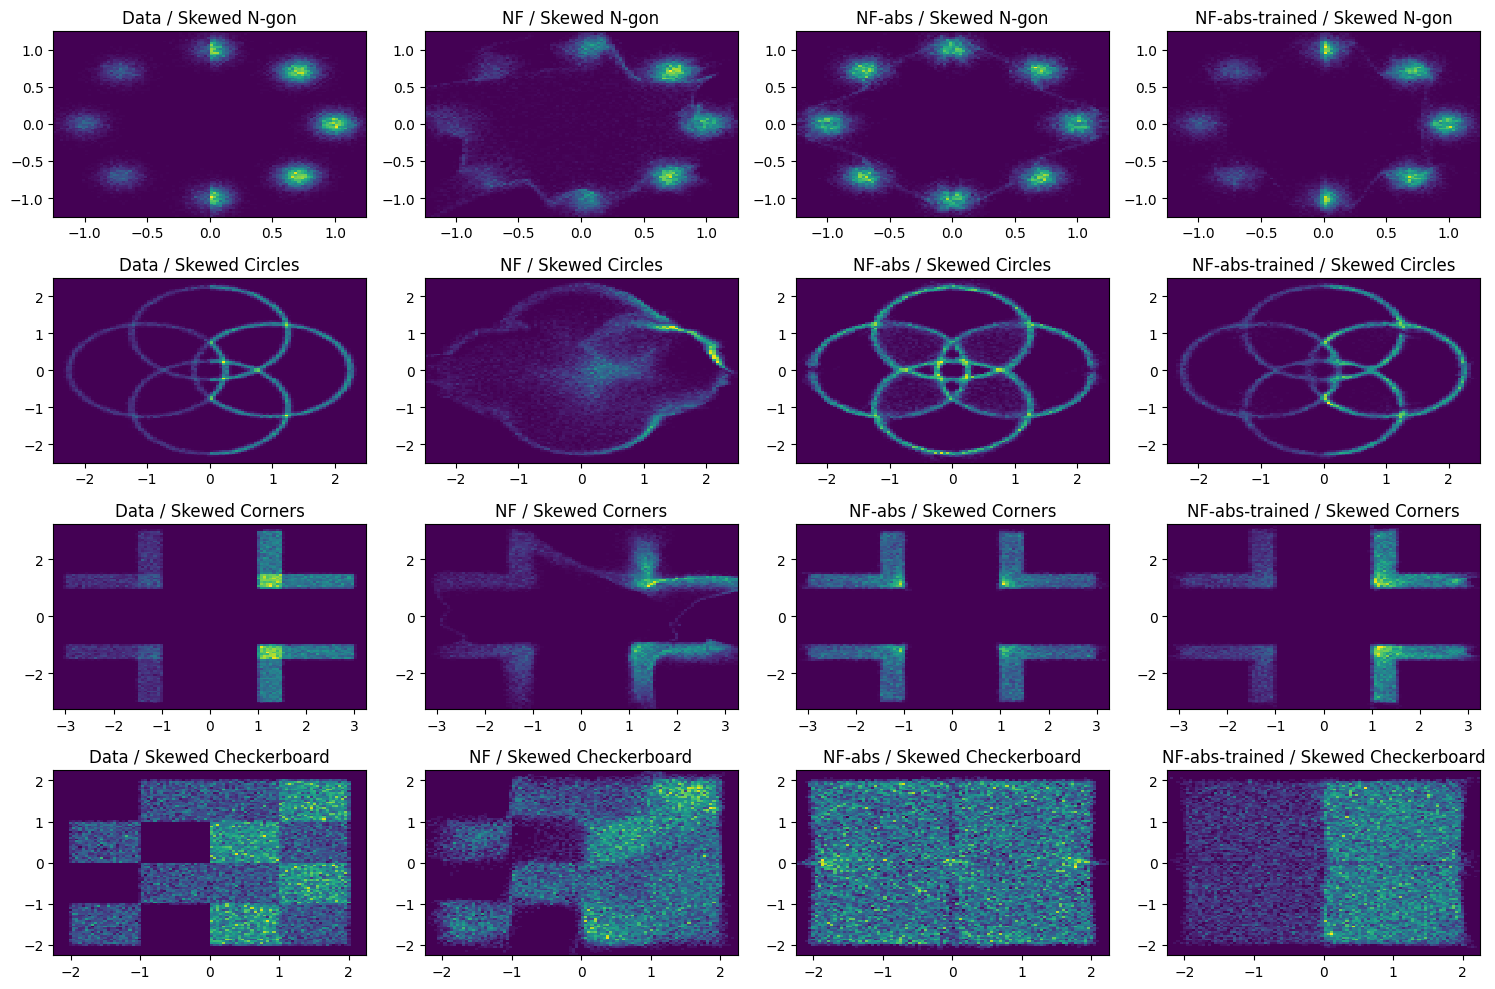
\includegraphics[width=.85\linewidth]{images/synthetic/abs-skewed.png}
    \caption{Comparison of methods for \textit{skewed} synthetic datasets; columns are same as Figure \ref{fig:abs-default}.}
    \label{fig:abs-skewed}
\end{figure}

\begin{figure}[H]
    \centering
    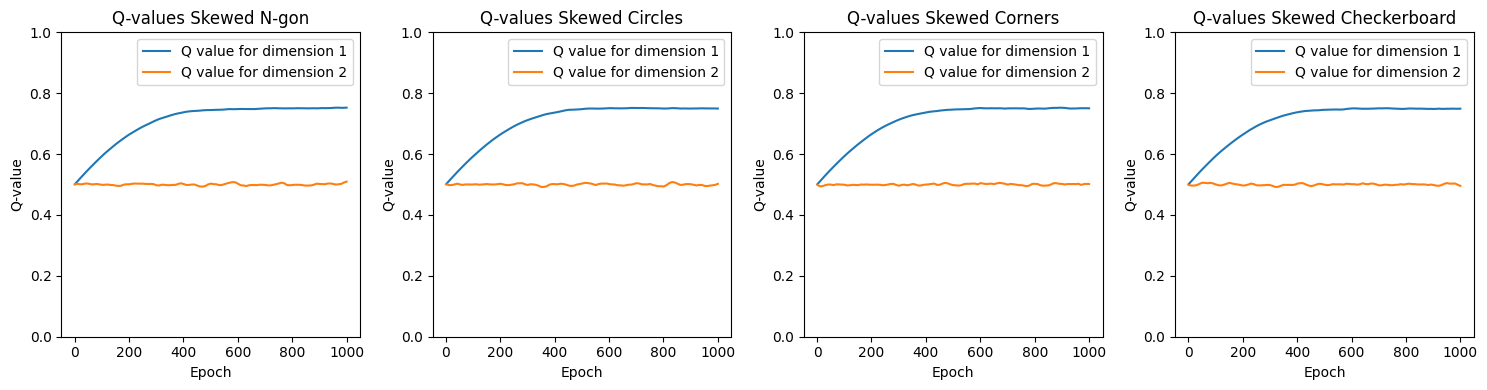
\includegraphics[width=.85\linewidth]{images/synthetic/skewed-q.png}
    \caption{Q-values for the last model of Figure \ref{fig:abs-skewed}.}
    \label{fig:skewed-q}
\end{figure}

The network indeed learns the correct Q-values of $0.75$ (since we flipped half of the data, i.e. the split becomes 25\%/75\%) for the $x$-axis, while the $y$-axis stays at $0.5$ (since it wasn't skewed).

Since this works well for a centered normalized dataset, the next step is to offset it by a constant (so the axes of symmetry are no longer the origin).  
The results can be seen in Figure \ref{fig:abs-offset}.

\begin{figure}[p]
    \centering
    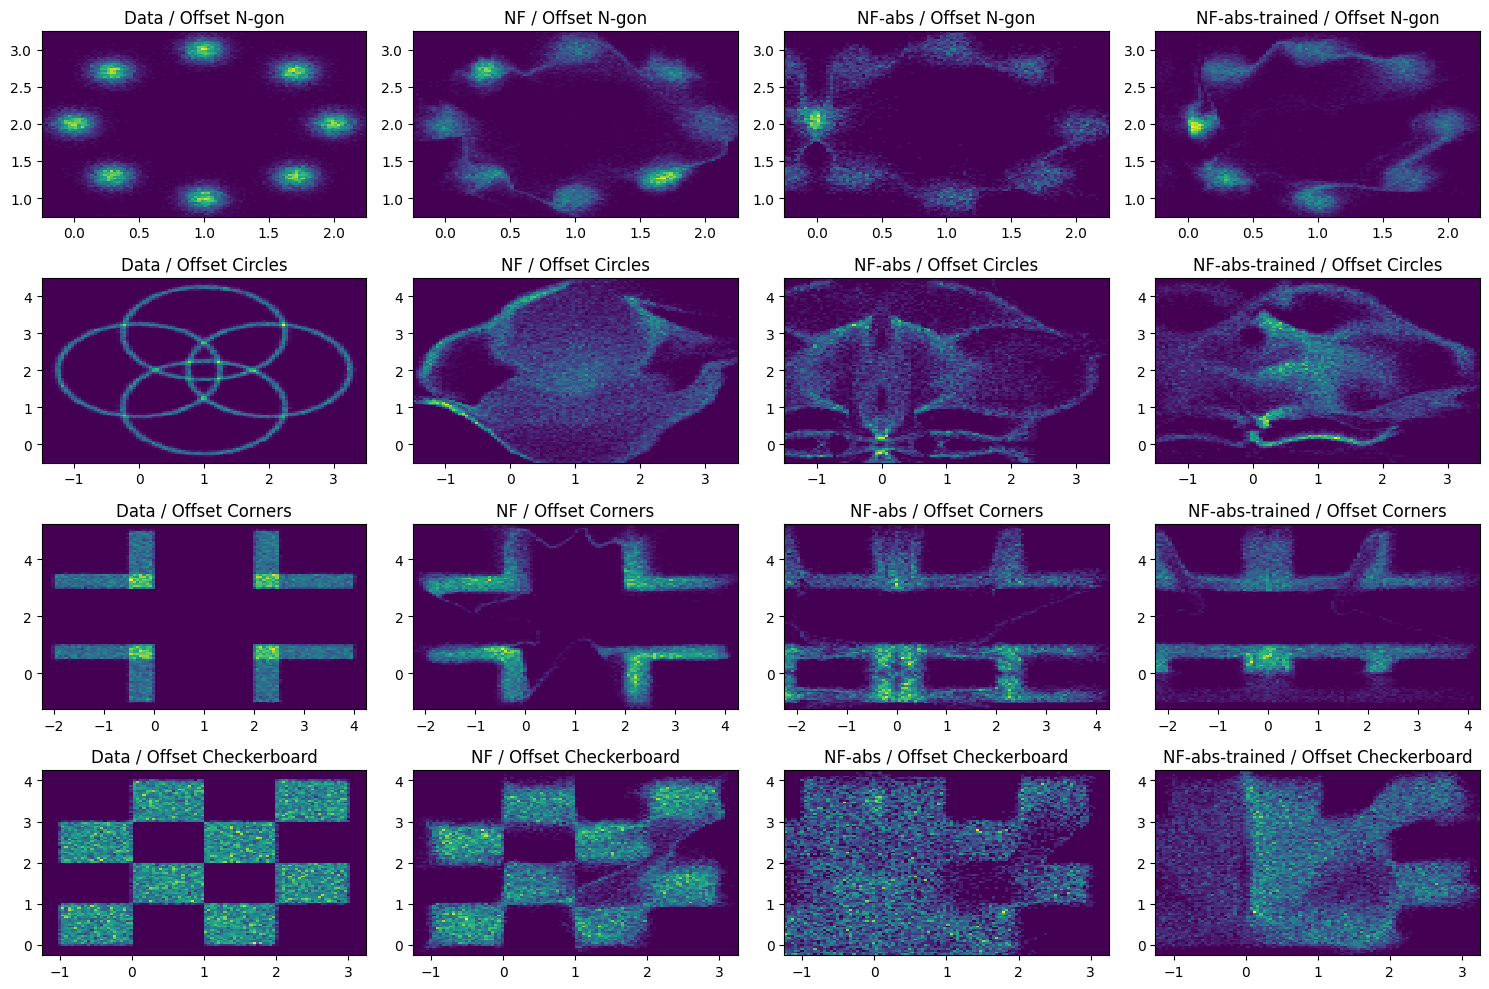
\includegraphics[width=.85\linewidth]{images/synthetic/abs-offset.png}
    \caption{Comparison of methods for \textit{offset} synthetic datasets; columns are same as Figure \ref{fig:abs-default}.}
    \label{fig:abs-offset}
\end{figure}

\begin{figure}[p]
    \centering
    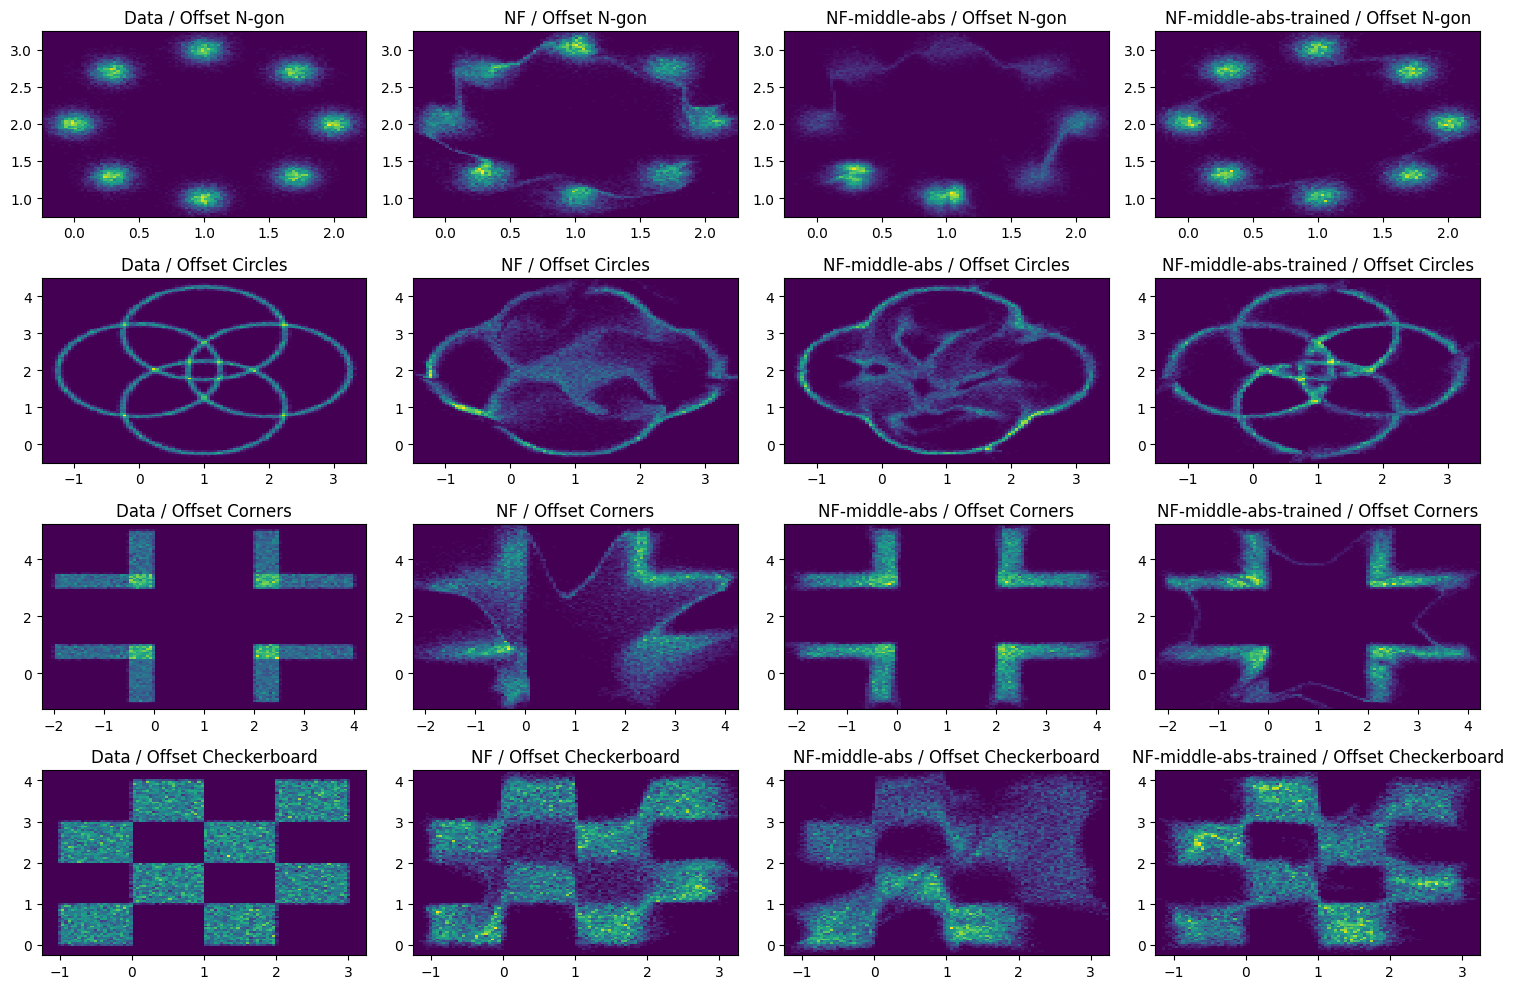
\includegraphics[width=.85\linewidth]{images/synthetic/abs-offset-fixed.png}
    \caption{Comparison of methods for \textit{offset} synthetic datasets; first two columns are same as Figure \ref{fig:abs-default}, last two are changed by moving the absolute layer in the middle.}
    \label{fig:abs-offset-fixed}
\end{figure}

Unsurprisingly, this breaks the architectures with an absolute layer at the beginning (which are the last two columns) since there are no layers after the mirroring happens to learn the offset.
This can be solved by changing the architecture to have the absolute layer in the middle so that the layers can learn the offset:

\begin{minted}{python}
(BijectiveLayer(2, [64] * 5), OrthonormalLayer(2)) x 5
AbsoluteLayer(2)
(BijectiveLayer(2, [64] * 5), OrthonormalLayer(2)) x 5
\end{minted}

The results can be seen in Figure \ref{fig:abs-offset-fixed}.

Doing this solves the problem and makes the models with the absolute layer (especially the last one; last column) perform much better for the synthetic datasets, which affirms the conclusion of the SurVAE paper regarding the usefulness of the \texttt{AbsoluteLayer} on symmetric data.

\asubsubsection{\texttt{AbsoluteLayer} -- Visualising symmetry axes}{Tomáš Sláma}

\textit{The results are taken from the \href{https://github.com/xiaoxiae/GNNFinal2024/blob/main/notebooks/abs.ipynb}{notebooks/abs.ipynb} notebook.}

Seeing that the models with the absolute layers performed well even on symmetric data with unaligned axes like the checkerboard, we wanted to see how the symmetries over the absolute layer looked like.

To visualize this, we trained multiple models for $1\,000$ epochs and then sent points along the axes of the latent space of the layer just behind the \texttt{AsoluteLayer} backwards through the layers. The results are visualized in Figures \ref{fig:symmetries_checkerboard} and \ref{fig:symmetries_checkerboard_2}. 

% \ref{fig:symmetries_all}. 
% \begin{figure}[h]
%     \centering
%     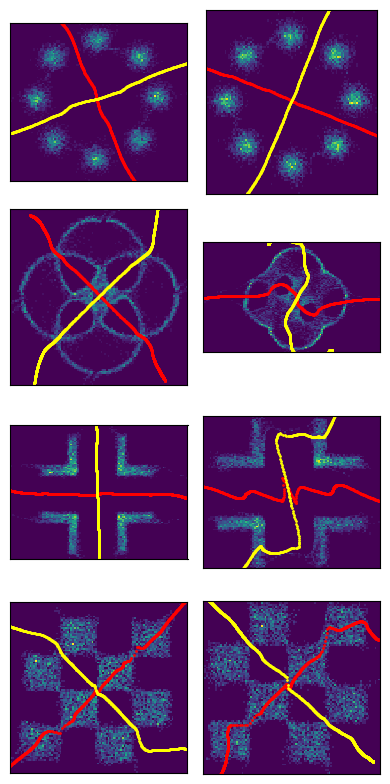
\includegraphics[angle=90, width=0.7\textwidth]{images/synthetic/symmetry_lines/symmetry_lines_all.png}
%     \caption{Symmetry lines from AbsoluteLayer for all datasets: first row is with learned q, second row with trained q}
%     \label{fig:symmetries_all}
% \end{figure}

\begin{figure}[H]
    \centering
    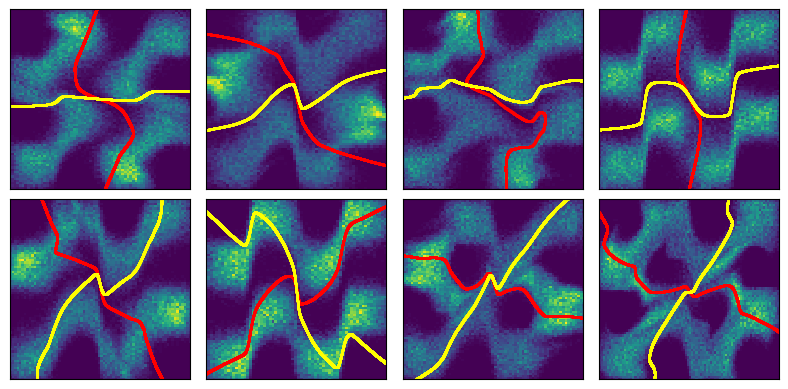
\includegraphics[width=0.9\textwidth]{images/synthetic/symmetry_lines/symmetry lines 3.png}
    \caption{Symmetry lines from \texttt{AbsoluteLayer} for Checkerboard after $100$ epochs. The symmetry lines are roughly correct and the datasets start to have the correct shape.}
    \label{fig:symmetries_checkerboard}
\end{figure}

\begin{figure}[H]
    \centering
    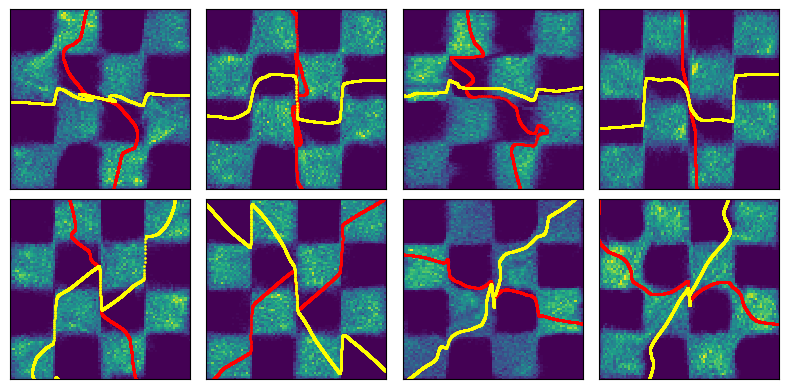
\includegraphics[width=0.9\textwidth]{images/synthetic/symmetry_lines/symmetry lines 4.png}
    \caption{Symmetry lines from \texttt{AbsoluteLayer} for Checkerboard after $1\,000$ epochs. Most of the datasets retain the original symmetry lines with only minor refinements, only one (row 1, column 2) changes them entirely.}
    \label{fig:symmetries_checkerboard_2}
\end{figure}

As we see, the learned symmetries are correct, albeit sometimes more complex than they need to be (diagonals would have sufficed).
They are also mostly unchanged after being established around $100$ epochs, just refined until the $1000$ epoch mark which contains correctly trained models. 

\asubsubsection{\texttt{AbsoluteLayer} -- Labeled}{Tomáš Sláma}

\textit{The results are taken from the \href{https://github.com/xiaoxiae/GNNFinal2024/blob/main/notebooks/abs\_conditional.ipynb}{notebooks/abs\_conditional.ipynb} notebook.}

Next, we took the labeled the datasets and modified the models to be conditional on the one-hot-encoding of the dataset labels.
Starting with the same models (baseline, abs, abs-trained) and datasets (n-gon, circles, corners, checkerboard) as the previous section, the results can be seen in Figure \ref{fig:abs-conditional}.

\begin{figure}[p]
    \centering
    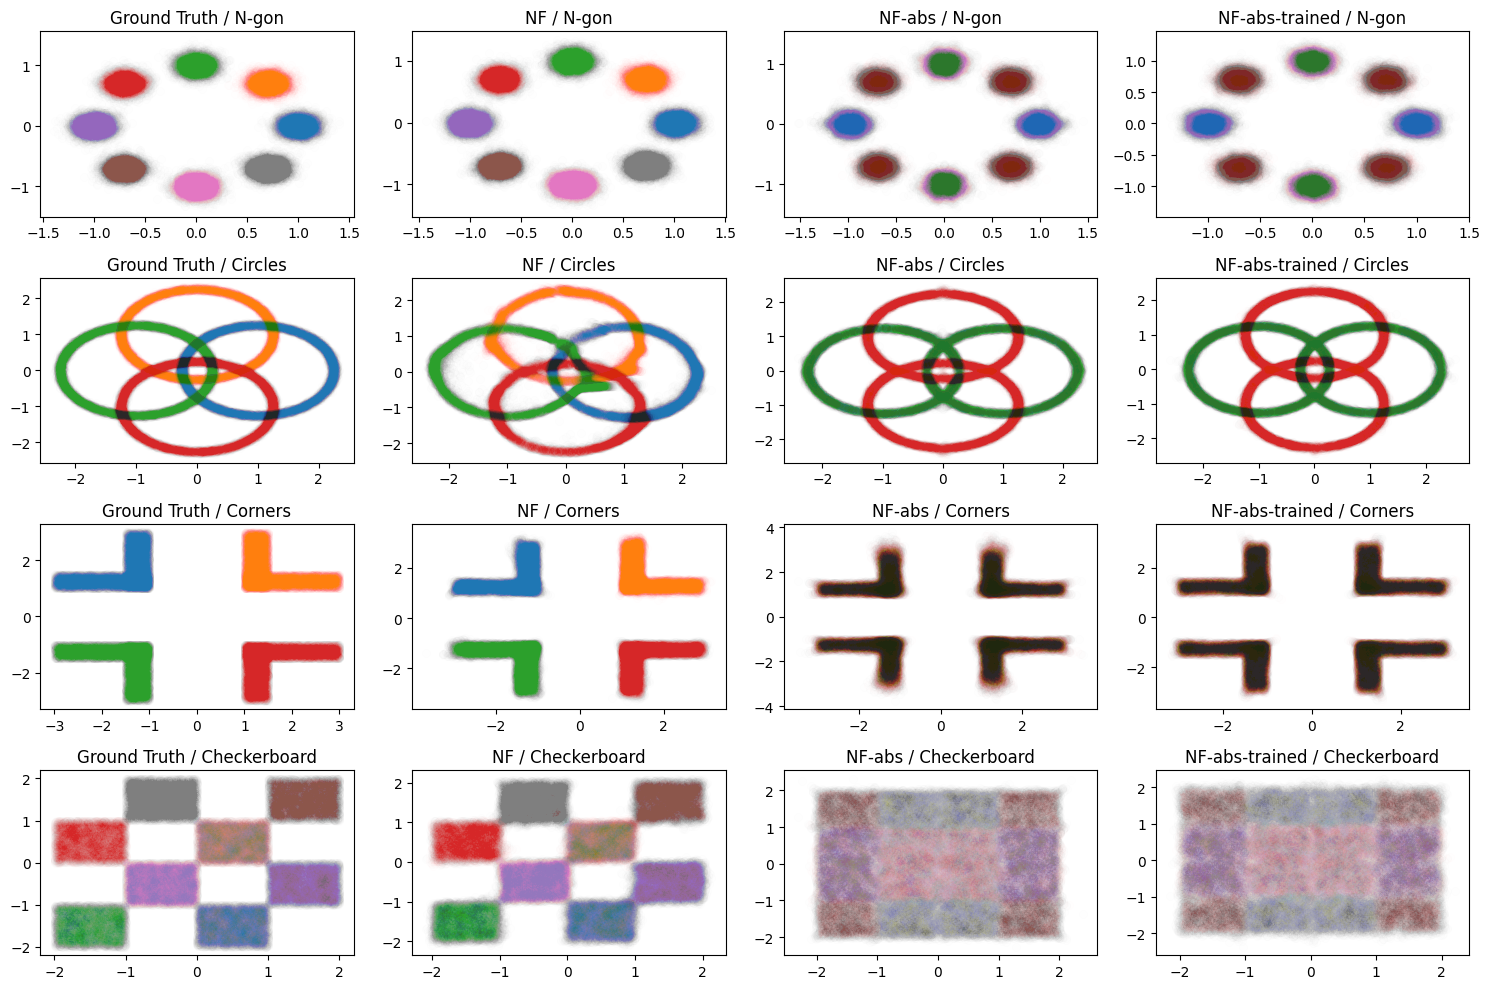
\includegraphics[width=.85\linewidth]{images/synthetic/abs-conditional.png}
    \caption{Comparison of methods for \textit{labeled} synthetic datasets; columns are same as Figure \ref{fig:abs-default}.}
    \label{fig:abs-conditional}
\end{figure}

\begin{figure}[p]
    \centering
    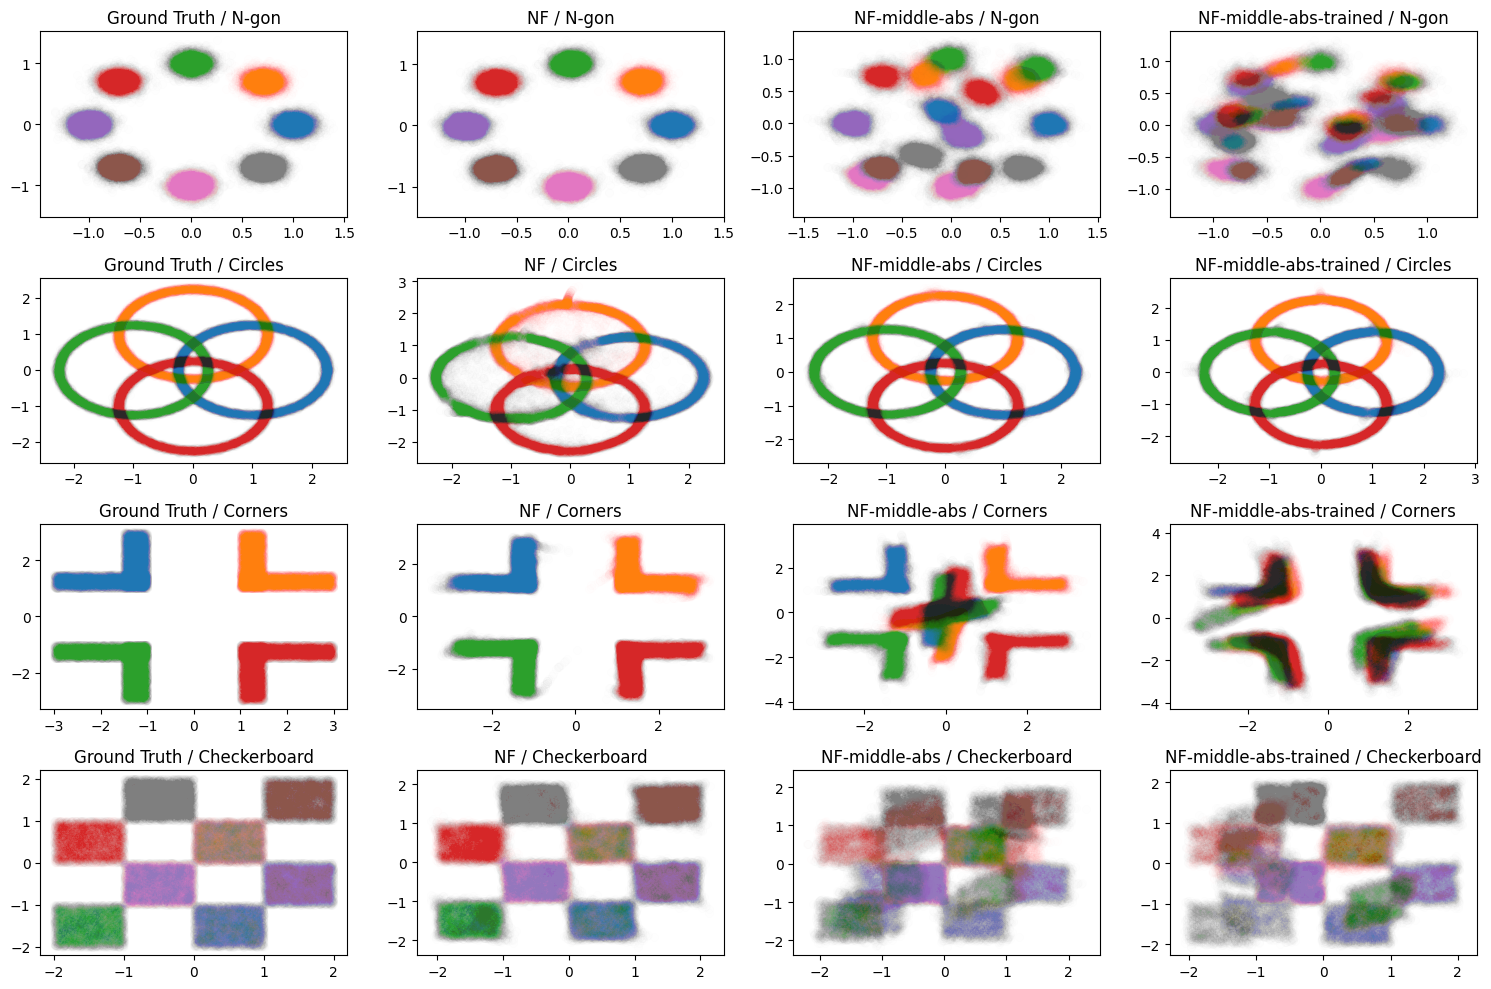
\includegraphics[width=.85\linewidth]{images/synthetic/abs-conditional-2.png}
    \caption{Comparison of methods for \textit{labeled} synthetic datasets; first two columns are same as Figure \ref{fig:abs-conditional}, last two are changed by moving the absolute layer in the middle.}
    \label{fig:abs-conditional-2}
\end{figure}


The models with the absolute layers suddenly become unusable, due to the fact that the datasets lose their symmetry. This is not solved by moving the absolute layer to the middle, as Figure \ref{fig:abs-conditional-2} shows.
\asubsubsection{\texttt{AugmentLayer}
-- Unlabeled}{Tomáš Sláma}

\textit{The results are taken from the \href{https://github.com/xiaoxiae/GNNFinal2024/blob/main/notebooks/augment.ipynb}{notebooks/augment.ipynb} notebook.}

The next experiment we chose to replicate is contained in appendix H.1 of the original paper, which compares a baseline normalizing flows network:

\begin{minted}{python}
(BijectiveLayer(2, [64] * 5), OrthonormalLayer(2)) x 3
BijectiveLayer(2, [64] * 5)
\end{minted}

with one that contains an \texttt{AugmentLayer} at the very beginning to make the dimensionality of all layers besides the last one increased:

\begin{minted}{python}
Augment(2, 4),
(BijectiveLayer(4, [64] * 5), OrthonormalLayer(4)) x 3
BijectiveLayer(4, [64] * 5)
\end{minted}

This should theoretically lead to better convergence, since the layers have more dimensions in which to optimize for the training values.
The results can be seen in Figure \ref{fig:augment}.

\begin{figure}[H]
    \centering
    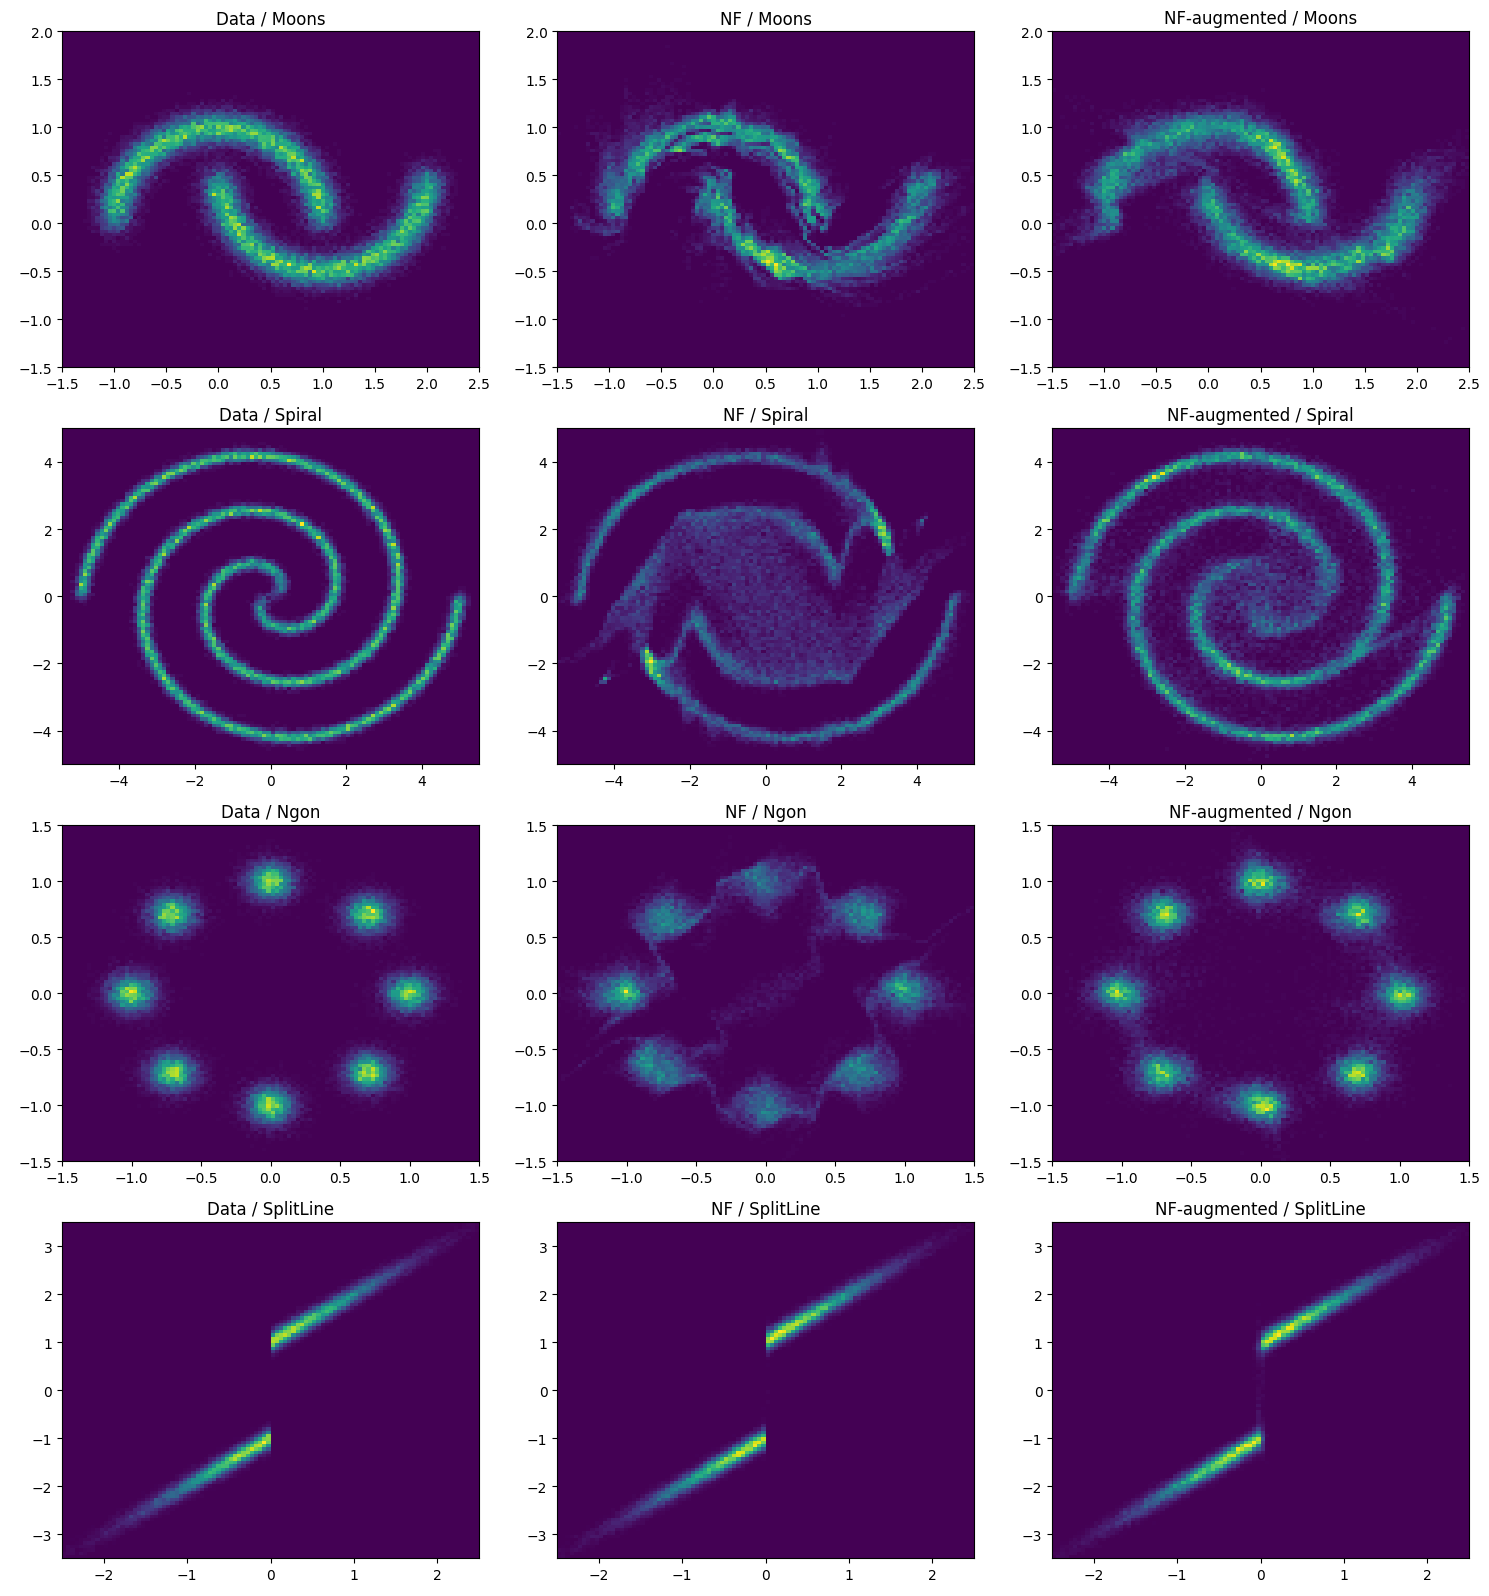
\includegraphics[width=.85\linewidth]{images/synthetic/augment.png}
    \caption{Five synthetic datasets (left column), along with a baseline NF network (middle column) and a network with an \texttt{AugmentLayer} at the beginning (right column).}
    \label{fig:augment}
\end{figure}

This is indeed the case and confirms the findings of the original paper.

\newpage

\asubsection{Point Cloud Data}{Maria Stickel}\label{sec:spatial_mnist}

\begin{figure}[p]
\centering
\begin{subfigure}[t]{.48\textwidth}
    \centering
    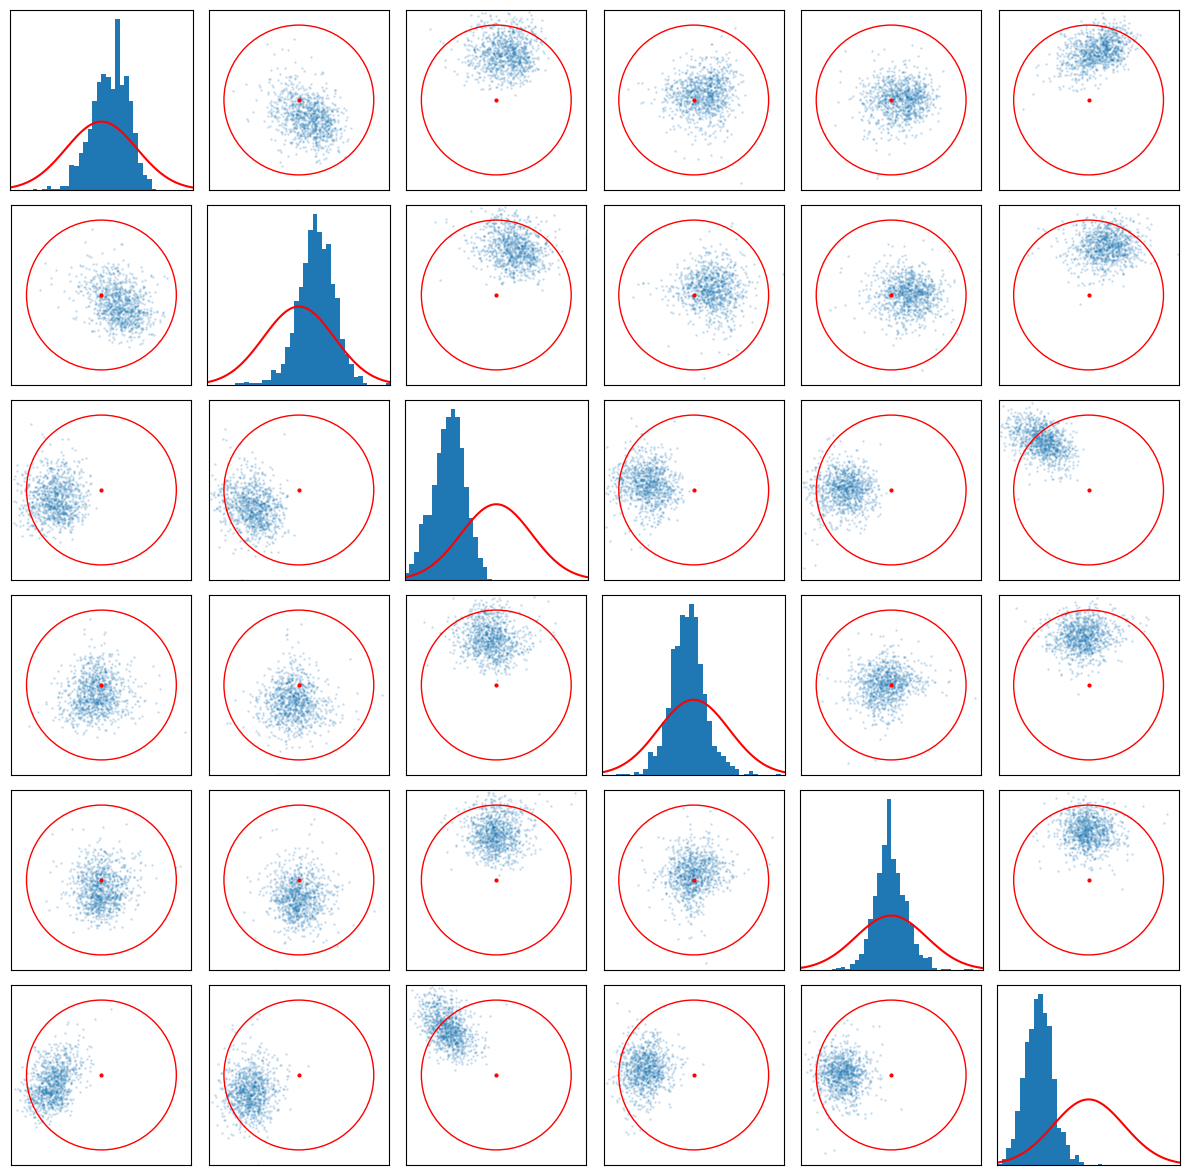
\includegraphics[width=\textwidth]{images/spatial_mnist/before_bij_layer_fix/calibration.png}
    \caption{One- and two-dimensional slices of the (N\textunderscore POINTS x 2)-dimensional latent distribution for the MNIST Point Cloud.}\label{fig:calibration_spatial_mnist_before}
\end{subfigure}
\hfill
\begin{subfigure}[t]{.48\textwidth}
    \centering
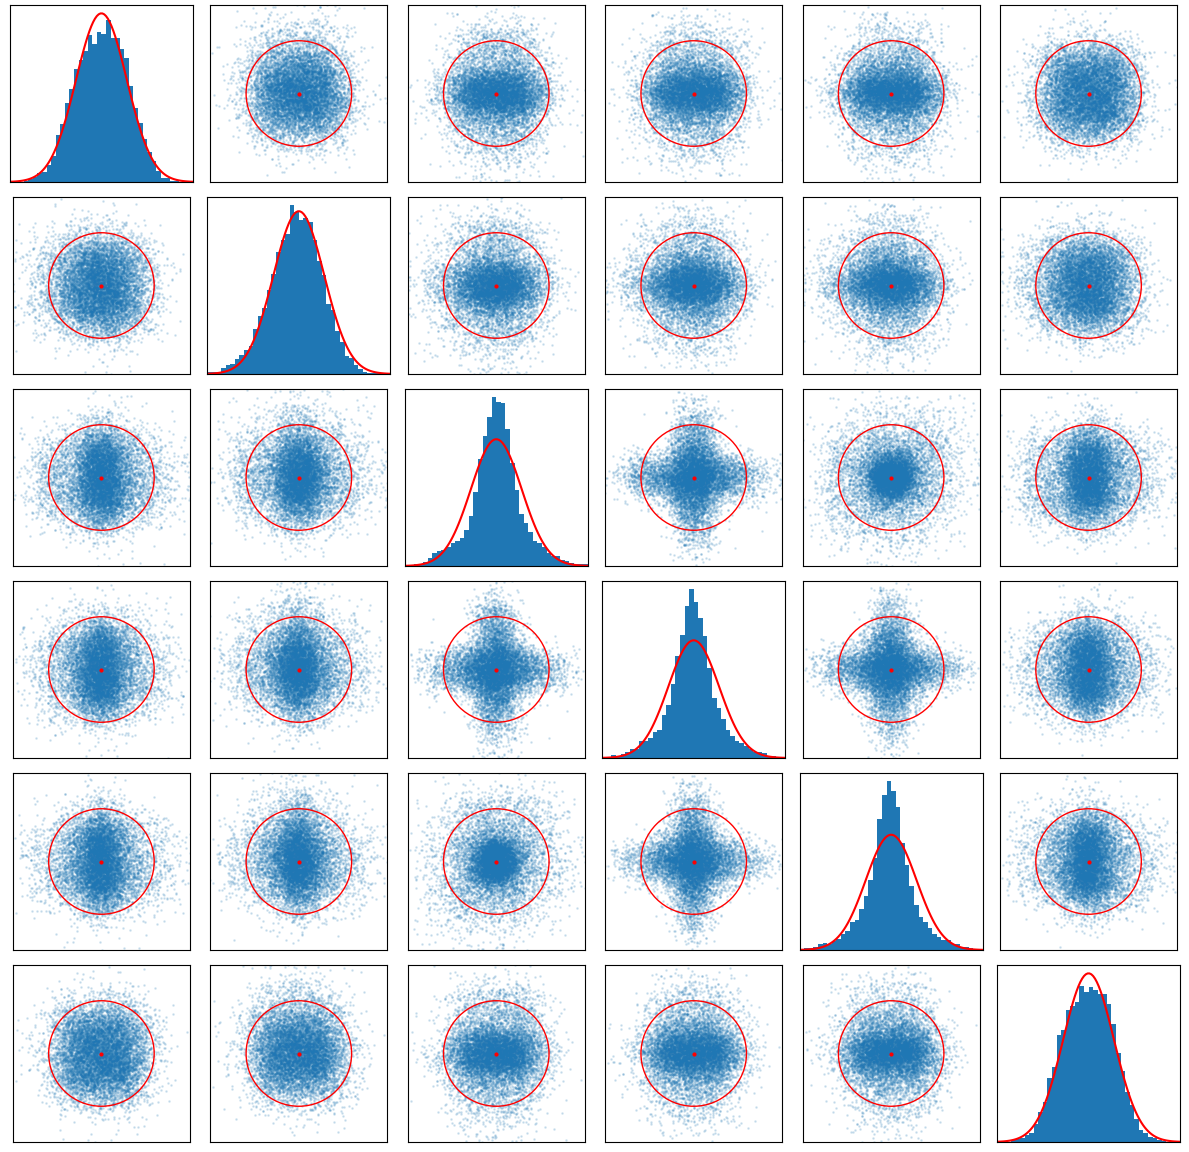
\includegraphics[width=\textwidth]{images/spatial_mnist/after_bij_layer_fix/code distribution.png}
    \caption{Code distribution for spatial MNIST after fixing the bijective layer.}
    \label{fig:spatial_mnist_code_after}
\end{subfigure}
\caption{Code distributions of SpatialMNIST model.}
\end{figure}

\begin{figure}[p]
    \centering
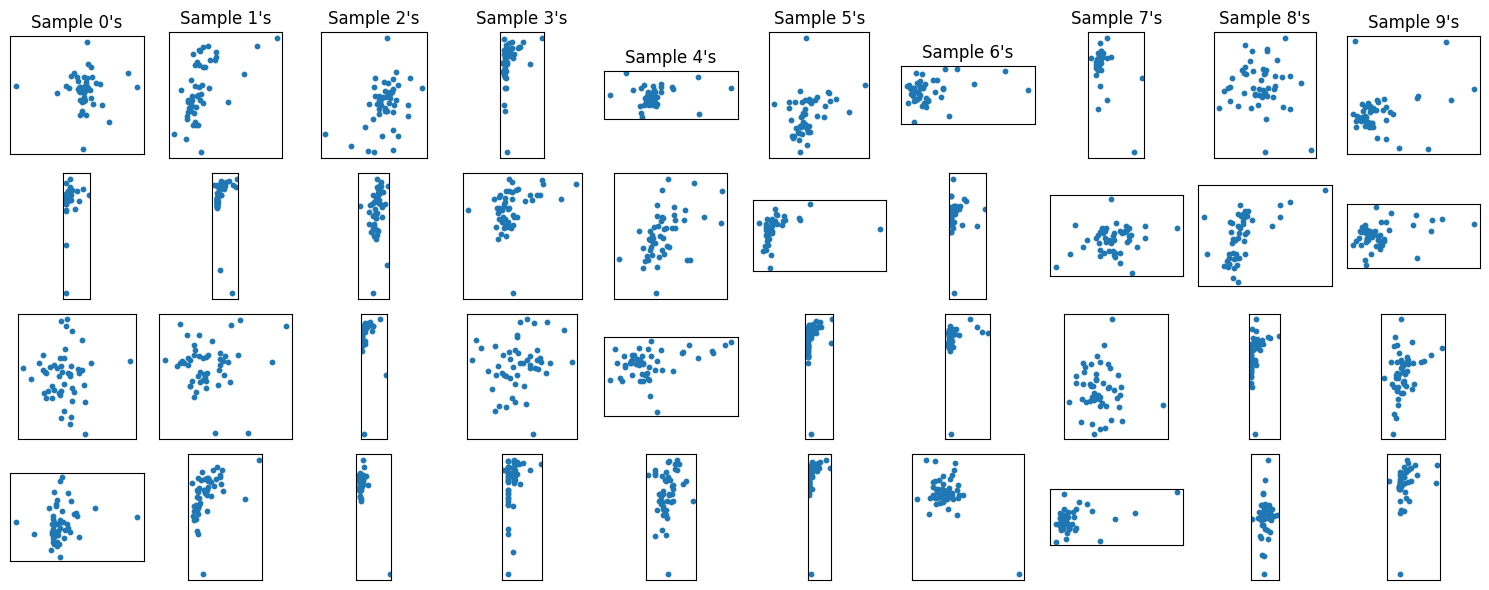
\includegraphics[width=0.95\textwidth]{images/spatial_mnist/after_bij_layer_fix/samples no ticks.png}
    \caption{Samples of our final spatial MNIST model}
    \label{fig:spatial_mnist_samples}
\end{figure}

\textit{The results are taken from the \href{https://github.com/xiaoxiae/GNNFinal2024/blob/main/notebooks/spatial_mnist.ipynb}{notebooks/spatial\textunderscore mnist.ipynb} notebook.}

\cite{nielsen2020survae} use parametrization by transformer networks (\cite{vaswani2023attention}) in their model architecture for the Point Cloud Data. As previously mentioned, we did not implement this feature, as we lack the knowledge about transformers (or rather the time to acquire a sufficient background of knowledge about their structure and application). We spent some time on researching transformer architectures, which the paper mentions in two (!) sentences without any further explanation of how they are applied in the architecture, although they used their own modified implementation for it. This research is not part of our architecture due to the fact that none of us have actually worked with transformers before and it proved to be too big of a topic to be learned and implemented that quickly. We thought about copying their transformer implementation, but using foreign code with nearly no knowledge on the underlying model is not a thing we wanted to do in a scientific research project.

We tried a different approach that didn't prove to be nearly as good as the paper, but then again, we ran into time issues. We report the results of our models. In the end, we decided to use the following architecture
\begin{minted}{python}
(
    PermuteAxesLayer((1, 0)), 
    BijectiveLayer((2, N_POINTS), [200, 200]), 
    PermuteAxesLayer((1, 0)),
    TranspositionLayer, 
    BijectiveLayer((N_POINTS, 2), [200, 200]), 
    PermutationLayer()
)   x 32,
ReshapeLayer((2, N_POINTS), (2 * N_POINTS,))
\end{minted}
where N\textunderscore POINTS is the number of points in the cloud. In each block we firstly permute in the first axis, i.e. re-order the list of points in the cloud. We apply a bijective transformation and permute again. Then we transpose the individual points in the cloud to ensure that the subsequent bijective transformation is applied on the vector entries skipped before (coordinate-wise). Another permutation completes the block. We reshape the data to enable easy sampling.

Before adjusting the bijective layer to this type of structured data, the results were bad. The standard deviation of the code distribution was measured to be 0.3879 which also aligns with the bad results shown in \ref{fig:calibration_spatial_mnist_before}. It should fulfill sigma=1, but one can only wonder whether this could have been achieved through more training with such an unfit model. The samples were equally bad.

Fixing the bijective layer and training in the architecture described above significantly improved the results. The code distribution resembles the normal distribution with sigma 1, see Figure \ref{fig:spatial_mnist_code_after}.

Training was done with the following hyperparameters:  batch-size=200, test-size=1\,000, epochs=100\,000 and initial learning rate=$10^{-3}$ with decay parameter gamma=0.97 applied every 1\,000 steps. The model in \cite{nielsen2020survae} was trained on a single GPU for 40 hours. The loss plot could lead one to think that the model has converged but could also be related to the learning rate decay. Needless to say we would have liked to train for a longer period and different hyperparameters, but there was no time. The model has not learned the distribution of the spatial MNIST dataset, see \ref{fig:spatial_mnist_samples}.


\asubsection{Image Data}{Jannis Heising}\label{sec:image_data}

\textit{The results were generated using the \href{https://github.com/xiaoxiae/GNNFinal2024/blob/main/notebooks/mnist784.ipynb}{notebooks/mnist784.ipynb} notebook.}

As with the preceding two sections, our initial goal was to replicate the paper's training setup as accurately as possible, i.e. to train a SurVAE with a dequantization layer and max-pooling layers on the CIFAR-10, ImageNet32, and ImageNet64 datasets. This was very ill-advised since the authors report a training time of two weeks for their simplest model, which was infeasible for our project, alas we only noticed the issue during the experiment setup. As a result, we chose to train a smaller SurVAE with similar architecture on a simpler dataset, namely MNIST784. As a benchmark, we planned to compare its FID score with state-of-the-art models for that dataset.

In contrast to the paper, we chose to make our model conditional, which was only feasible due to our simpler dataset. The condition is a one-hot encoding of the digits 0-9. This means that a fully trained model would be able to create images of specific digits as opposed to arbitrary ones.

We chose the following baseline architecture:

\begin{minted}{python}
DequantizationLayer(),
(BijectiveLayer(784, [200, 200]), OrthonormalLayer(784)) x 5,
MaxPoolingLayer(784, 2),
(BijectiveLayer(196, [200, 200]), OrthonormalLayer(196)) x 5,
MaxPoolingLayer(196, 2),
(BijectiveLayer(49, [200, 200]), OrthonormalLayer(49)) x 5,
MaxPoolingLayerWithOverlap(49, 3, 2),
(BijectiveLayer(9, [200, 200]), OrthonormalLayer(9)) x 5
\end{minted}

In other words, the model uses four different scales (28x28, 14x14, 7x7, 3x3) and 5 steps per scale, and all nested neural networks have two hidden layers of size 200. We chose to end up with a fairly low-dimensional latent distribution because the information contained in the images is very small - one of ten digits with slightly varying styles.

On the other hand, each downscaling step should be gentle in the sense that we do not want to loose too much data at once, hence four scales. The choice of twenty bijective layers was based on the assumption that the model could be slightly simpler than those described in the paper, which had twenty-four.\footnote{We only list the parameter choices we deem interesting here. The exact setups for the tests in this section are documented in the repository, should more detail be desired. They are always stored as ``\texttt{setup.txt}" in the appropriate directories.}

For proper hyperparameter testing, each choice of parameters should ideally be tested several times and updated systematically. However, the given time frame of three weeks did not allow for such rigorousness for a model of the given complexity. Thus, we properly tested each configuration only once (plus small preliminary tests of a few epochs each) and iteratively chose the next experiment mainly based on the outcome of its predecessor. A ``proper test" consisted of a training time of around eight hours on an Nvidia~GTX~970 graphics card.

\textbf{Experiment 1:} In our first attempt, we somewhat foolishly used a reconstruction loss term because the NLL loss for the max-pooling layers was implemented incorrectly. We also disabled the dequantization layer to make the reconstruction loss more expressive. The samples presented in Figure~\ref{fig:mnist_run_1_samples} show that this approach was unwise.

\textbf{Experiment 2:} After fixing the problematic NLL loss terms, we trained another model with the exact architecture shown above. The new samples (Figure~\ref{fig:mnist_run_2_samples}) seemed more promising, but still far from perfect. The drastic difference between the top and bottom halves of the sampled images stems from the first (i.e. last during generation) bijective layer, in which the upper half constitutes the skip connection and only the lower half is altered. This perhaps suggests that the layer in question is being trained much more slowly than the other ones, although we were unable to find a cause for such a phenomenon. Furthermore, while the learned latent distribution did resemble a normal distribution, it had the wrong standard deviation, as shown in Figure~\ref{fig:mnist_run_2_latent_distr}. At any rate, the loss graph (Figure~\ref{fig:run_2_loss}) seemed to suggest that this model had reached its peak.

\begin{figure}
\centering
\begin{subfigure}[t]{.48\textwidth}
    \centering
    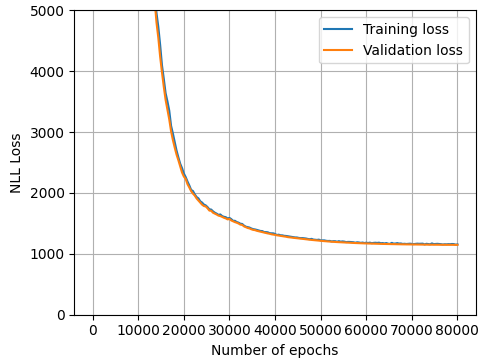
\includegraphics[width=\textwidth]{images/mnist_maxpooling/run_2_loss.png}
    \caption{Loss graph of the second experiment. The model seems to have mostly stagnated.}
    \label{fig:run_2_loss}
\end{subfigure}
\hfill
\begin{subfigure}[t]{.48\textwidth}
    \centering
    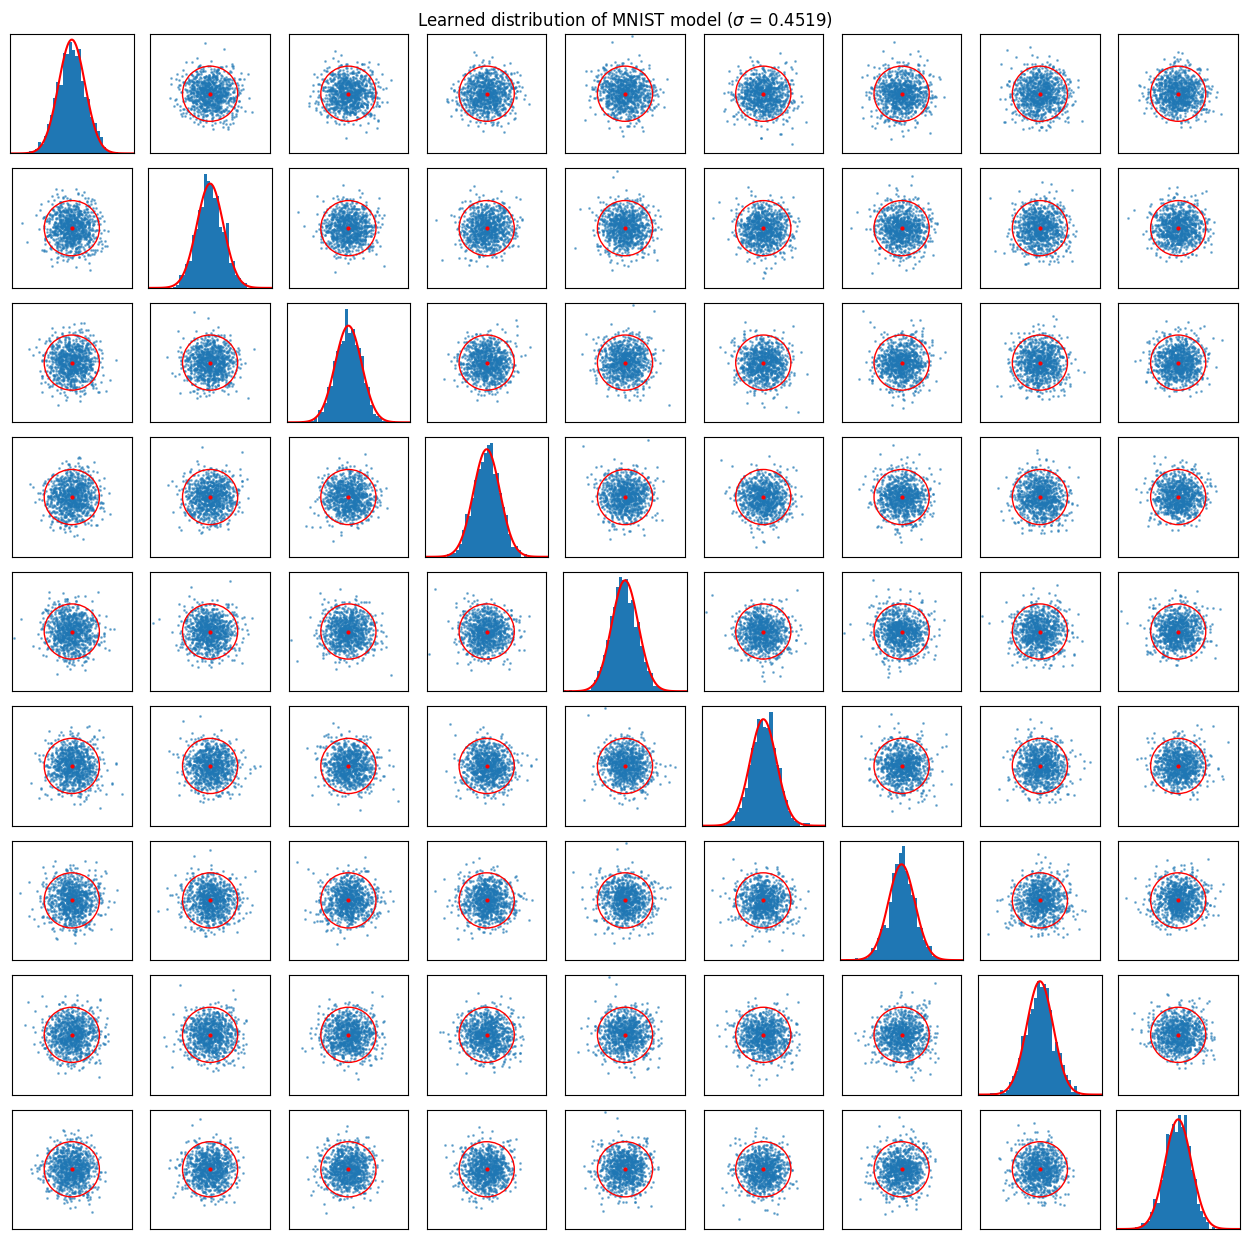
\includegraphics[width=.8\textwidth]{images/mnist_maxpooling/run_2_latent_distr.png}
    \caption{One- and two-dimensional slices of the nine-dimensional latent distribution. It clearly resembles a normal distribution with standard deviation around 0.45 (shown in red; the circles indicate the 90\%-threshold) instead of the desired 1.}
    \label{fig:mnist_run_2_latent_distr}
\end{subfigure}
\caption{Results from experiment 2.}
\end{figure}

\textbf{Experiment 3:} Next, we increased the model architecture to six steps per scale (instead of five) and increased the hidden layer sizes of the nested neural networks in the first scale to \verb|[200, 500, 200]| (from \verb|[200, 200]|). In an attempt to speed-up training, we decreased the hidden layer sizes in the last scale to \verb|[200]| (from \verb|[200, 200]|). Figure~\ref{fig:mnist_run_3_samples} illustrates that these changes did not help.

While our previous attempts at explaining either of the two major problems of the second test - slow \texttt{BijectiveLayer} training and small standard deviation - were fruitless, we now managed to trace both back to the same root cause. We want to explain how we actually found the issue in the hopes that it might help readers when debugging their own implementation. To start, let us take another look at the NLL loss (cf. Section~\ref{sec:nf_explanation}):

\begin{align*}
\text{NLL} &= \mathbb{E}_{X \sim p^*(X)} [-\log(p(X))]\\
&= \mathbb{E}_{X \sim p^*(X)} [-\log(q(f(X) \cdot |\det \mathcal{J}_{f}|)]\\
&\approx \underbrace{- \frac{1}{N} \sum_{i=1}^N \log(q(f(X_i))}_{=: A} - \underbrace{\frac{1}{N} \sum_{i=1}^N \log(|\det \mathcal{J}_{f, i}|)}_{=: B}
\end{align*}

Roughly speaking, term $A$ is responsible for pulling samples in the code distribution towards the origin, whereas term $B$ makes sure the translation between latent and data distribution is good. Seeing that our model excelled at the former and struggled with the latter, we were confident that the balance between the two was off. Term $A$ is very simple and was quickly ruled out as the culprit. Thus, we revisited term $B$, i.e. the log-likelihood computation of the layers. As we had similar problems with other experiments that did not involve max-pooling layers, it was clear that the issue had to lie within the \texttt{BijectiveLayer} class. Carefully examining our implementation, we realized that our coefficient generation was faulty. Recall that the bijective layer performs a computation of the form (cf. Section~\ref{sec:bijective})

\[
\tilde{X} = s \cdot X + t,
\]

where the coefficients $s$ and $t$ are the output of a feed-forward neural network. The shape of the vector $X$ is \verb|(N, D)|, where $N$ is the batch size and $D$ is the data size. It should be clear that $s$ and $t$ ought to have the same shape, however we only sampled $s$ of shape \verb|(N, 1)|, i.e. we applied the same coefficient to all data dimensions for each batch entry. This alone is quite bad as it greatly limits the transformative power of the layer, but it wouldn't have caused the issues we observed, had we not simultaneously assumed for the log-likelihood computation that $s$ has the correct shape. This resulted in the log-likelihood term being $D$ times too small, creating the aforementioned imbalance between the loss terms $A$ and $B$.

\textbf{Experiment 4:} Having resolved this slight inconvenience, we repeated the setup of the second test as it had yielded the best results up to that point. However, we did change two parameters: Firstly, we decreased the batch size from 1,000 to 200. Both of these values were chosen rather arbitrarily as we did not have the time to conduct rigorous hyperparameter test as mentioned above. The decrease massively sped up training, going from roughly 2.8 to just over 8.2 epochs per second, and seemed not to dampen the training merit of each epoch in equal and opposite magnitude, in other words it was an unequivocally good change. Secondly, we increased training time from around 8 to 11 hours split into sessions of 3 and 8 hours. This change stemmed from the general principle that ``more training is better" and the fact that our schedules happened to allow for the additional training.

Disappointingly, the samples (Figure~\ref{fig:mnist_run_4_samples}) were still bad, but we did find a plausible explanation for it: Throughout all of these experiments, we had been using learning rate decay and basically eyeballing the values for it.\footnote{Again, the exact values are recorded in the repository.} When plotting the learning rate together with the test loss during training (Figure~\ref{fig:mnist_run_4_loss_vs_lr}), one senses a strong correlation between the two.

\begin{figure}
\centering
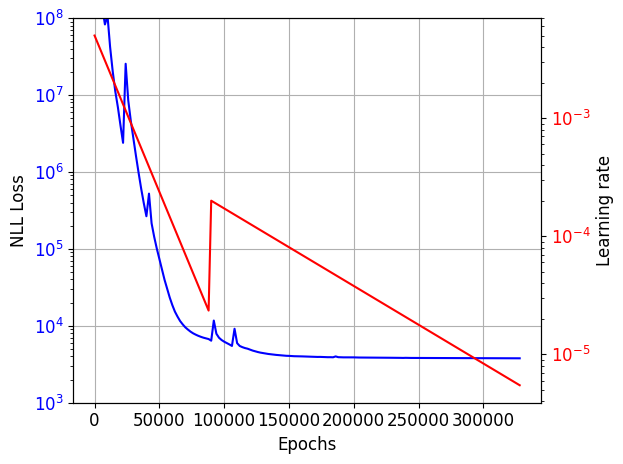
\includegraphics[width=.65\textwidth]{images/mnist_maxpooling/run_4_loss_vs_lr.png}
\caption{Negative log-likelihood loss (blue, log-scale) and learning rate (red, log-scale) from the fourth test. The irregularity in both lines at 88,000 epochs indicates the start of the second training session. The somewhat faster loss decrease right afterwards seems to stem from the increased learning rate.}
\label{fig:mnist_run_4_loss_vs_lr}
\end{figure}

\begin{figure}
\centering
\begin{subfigure}[t]{0.45\textwidth}
    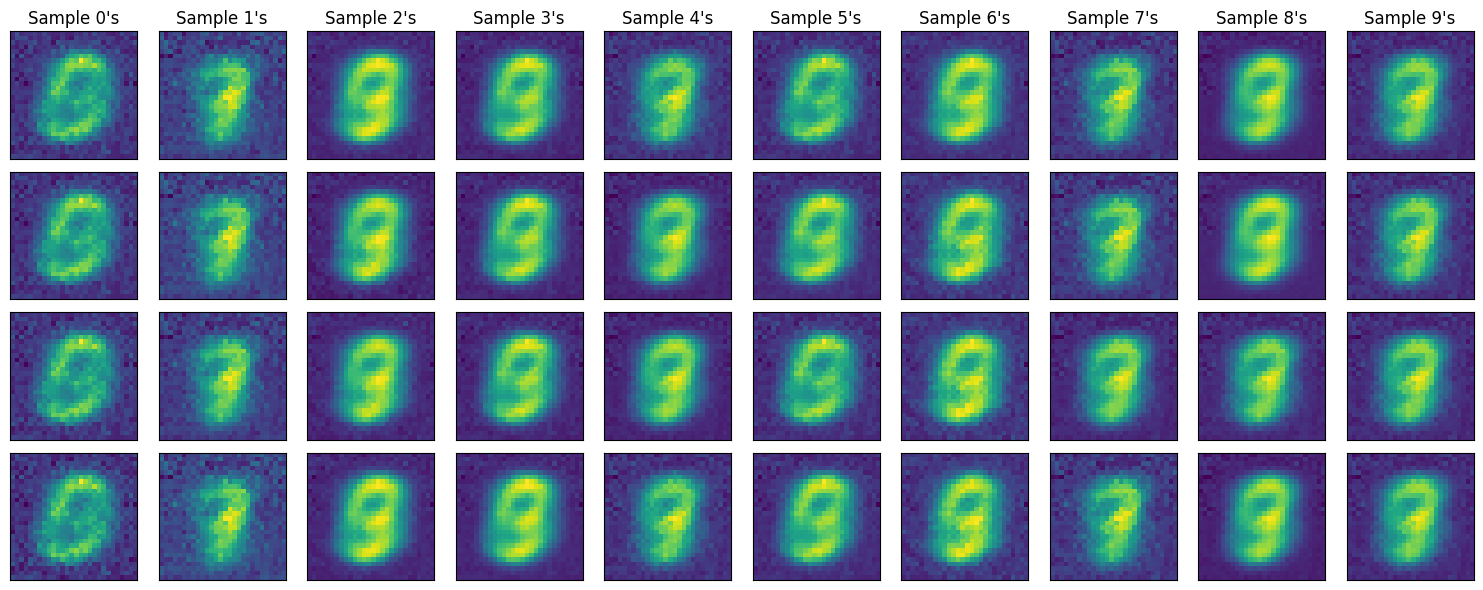
\includegraphics[width=\textwidth]{images/mnist_maxpooling/run_1_samples.png}
    \caption{\footnotesize Samples from the first experiment. Each digit (column) was sampled four times (row). The images are barely distinguishable and mostly resemble a blur of all digits.}
    \label{fig:mnist_run_1_samples}
\end{subfigure}
\hfill
\begin{subfigure}[t]{0.45\textwidth}
    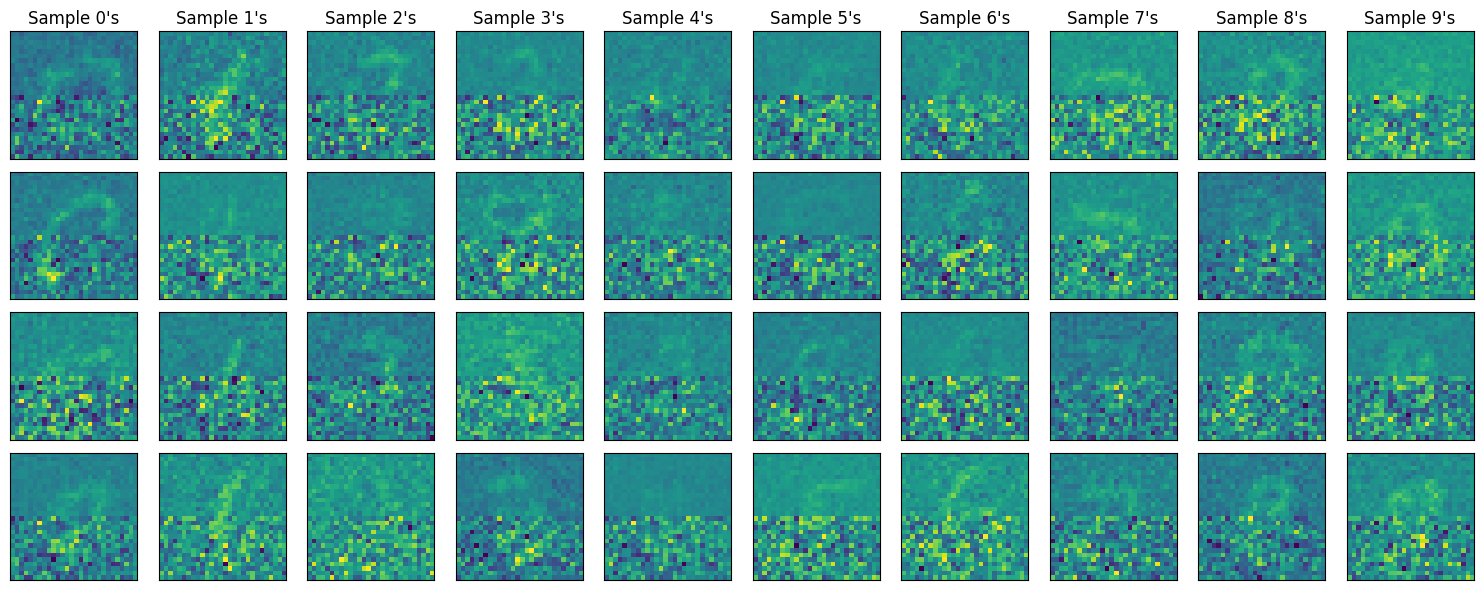
\includegraphics[width=\textwidth]{images/mnist_maxpooling/run_2_samples.png}
    \caption{\footnotesize Samples from the second experiment. The images are split in-two, with the top half showing vaguely correct shapes and the lower half being mostly gibberish.}
    \label{fig:mnist_run_2_samples}
\end{subfigure}\\
\vspace{.5em}
\begin{subfigure}[t]{0.45\textwidth}
    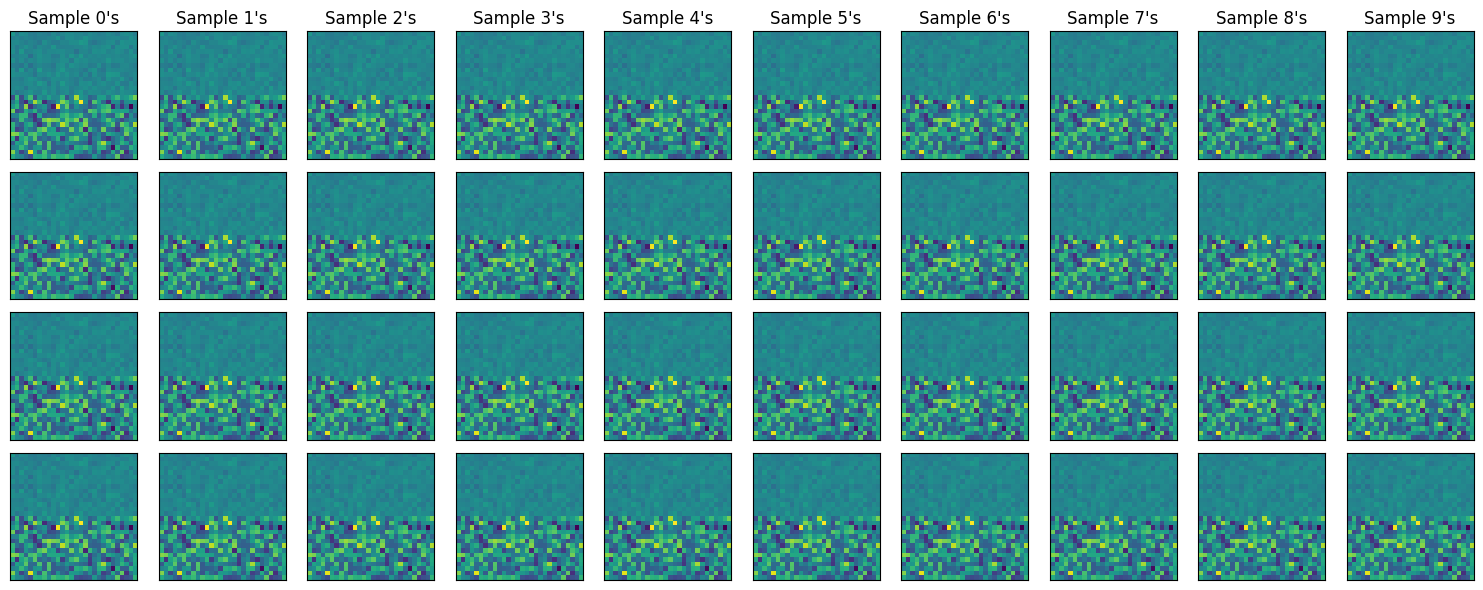
\includegraphics[width=\textwidth]{images/mnist_maxpooling/run_3_samples.png}
    \caption{\footnotesize Samples from the third experiment. The model did not converge after eight hours of training and the half-split conundrum persists.}
    \label{fig:mnist_run_3_samples}
\end{subfigure}
\hfill
\begin{subfigure}[t]{0.45\textwidth}
    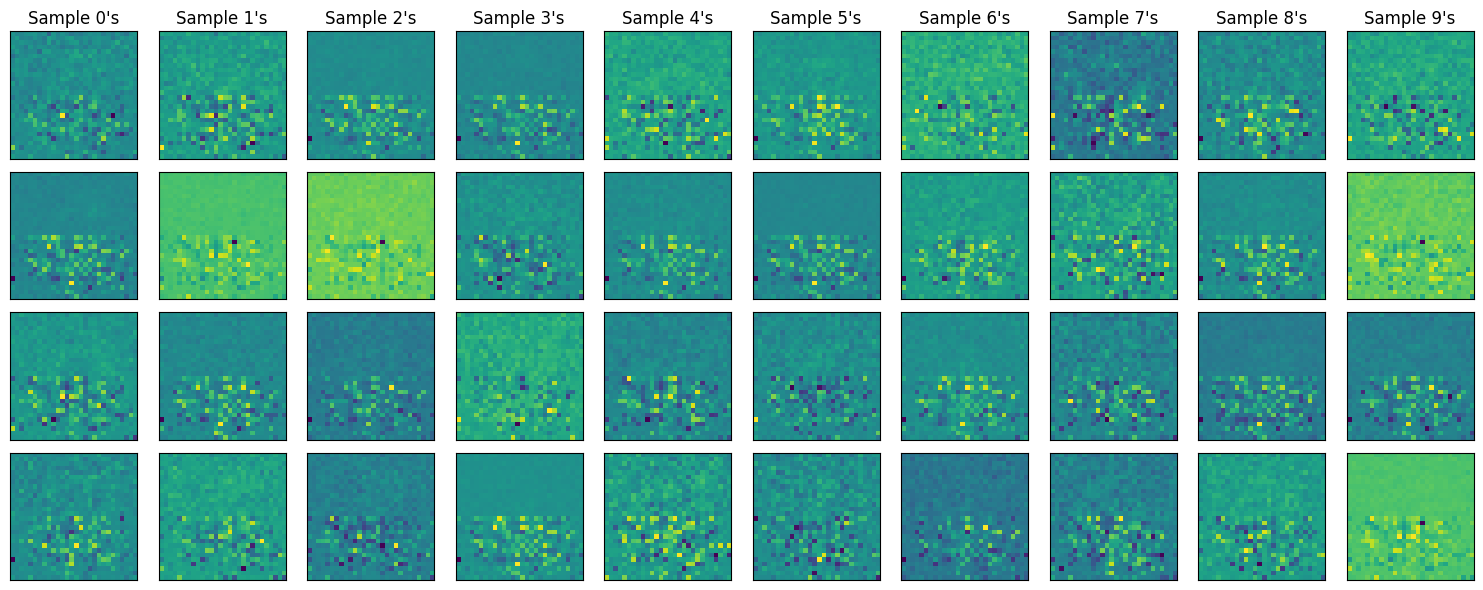
\includegraphics[width=\textwidth]{images/mnist_maxpooling/run_4_samples.png}
    \caption{\footnotesize Samples from the fourth experiment. There is no trace of digit shapes and the samples are still bi-regional, although notably less so.}
    \label{fig:mnist_run_4_samples}
\end{subfigure}
\caption{Samples from the MNIST experiments.}
\label{fig:mnist-all-samples}
\end{figure}

\textbf{Experiment 5:} From Figure~\ref{fig:mnist_run_4_samples}, we deduced that a constant learning rate of $10^{-4}$ should be ideal. We chose the model trained for 50,000 epochs from the previous test as the starting point for training and kept all other parameters as before. Figure~\ref{fig:mnist_4_vs_5} illustrates the impact of the higher learning rate: Initially, the model did learn faster, however its final performance was only marginally better; its samples were indistinguishable from those of the previous experiment. Furthermore, training seemed to be less stable, with the loss curve exhibiting significantly more spikes than before.

\begin{figure}
\centering
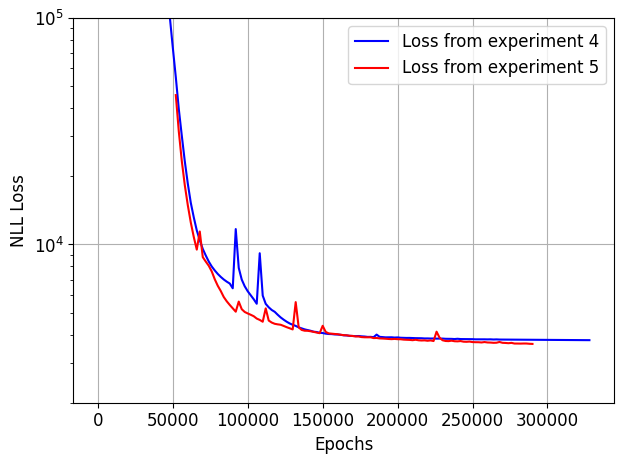
\includegraphics[width=.7\textwidth]{images/mnist_maxpooling/run_4_vs_5.png}
\caption{Validation loss from the fourth and fifth experiment.}
\label{fig:mnist_4_vs_5}
\end{figure}

From this result, we postulate that the chosen architecture was not expressive enough for the task. Unfortunately, we did not have time to conduct further experiments. Were we to resume our tests, we would like to use models with more bijective layers and larger nested networks, and we would like to measure how changing the latent dimensionality impacts the results.

It does not make sense to compare our work to the state-of-the-art using FID, seeing as our samples are unrecognizable.


\newpage
\asubsection{Parameter Degeneracy}{Jannis Heising}

Since this section explores an application of SurVAEs not discussed in the paper we are trying to replicate, the experiments described here were given less attention and, crucially, less time. As a result, many results are bad simply due to not being trained for long enough.

\asubsubsection{SBI}{Jannis Heising}\label{sec:sbi}

\textit{The results were generated using the \href{https://github.com/xiaoxiae/GNNFinal2024/blob/main/notebooks/sir.ipynb}{notebooks/sir.ipynb} notebook.}

The initial goal of our experiments involving parameter degeneracy was to assess whether the SurVAE architecture could be designed to cope with degenerate SBI models. To this end, we created a baseline by reimplementing exercise 1 from sheet 4 using both our own solution and snippets as well as general ideas from the sample solution. The exercise in question concerned the most basic SIR model described in Section~\ref{sec:sir_data}. We chose the following architecture for all experiments on this basic system:

\begin{minted}{python}
(BijectiveLayer(3, [150, 150]), OrthonormalLayer(3)) x 30
\end{minted}

Additionally, we equipped the SurVAE with a summary network $h$, which is a simple feed-forward neural network that condenses the conditional input - the observation data - into a more usable form for the SurVAE layers. We chose the layer sizes of $h$ to be \verb|[200, 200, 200, 100]| based on prior testing.

For the degenerate data, we replaced $\lambda$ by two new parameters $\lambda_1$ and $\lambda_2$ as explained in Section~\ref{sec:background_param_degen}. Initially we chose the exact same SurVAE architecture as before for this data, including that of the summary network, except that the bijective and orthonormal layers now act on four instead of three dimensions. This was to create a benchmark of how well the standard NF model performs on degenerate data to later compare to more sophisticated models.

\textbf{Experiment 1:} To get our bearings, we simply wanted to recreate the results from the exercise sheet and, ideally, show that the standard NF performed badly on degenerate data. We trained both the basic and the degenerate model (i.e. the model trained on the degenerate dataset) until convergence with underwhelming results.

The calibration diagrams and code distributions (Figure~\ref{fig:sir_run_1}) show that our models did not learn the correct distribution. As it turned out, this test used the faulty implementation of the \texttt{BijectiveLayer} as discussed in Section~\ref{sec:image_data}, so bad results were to be expected.

\begin{figure}[t]
\centering
\begin{subfigure}{\textwidth}
    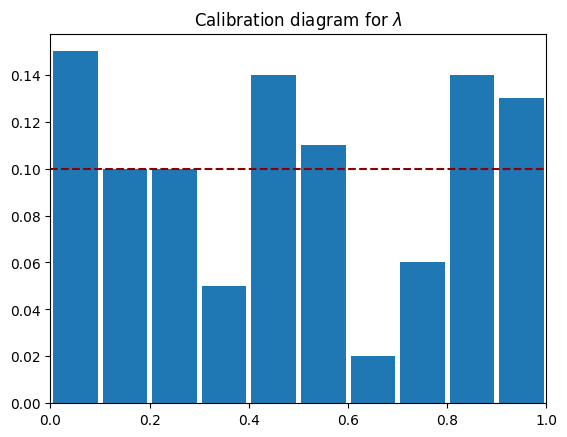
\includegraphics[width=.23\textwidth]{images/sbi_sir/run_1/basic calib lambda.png}
    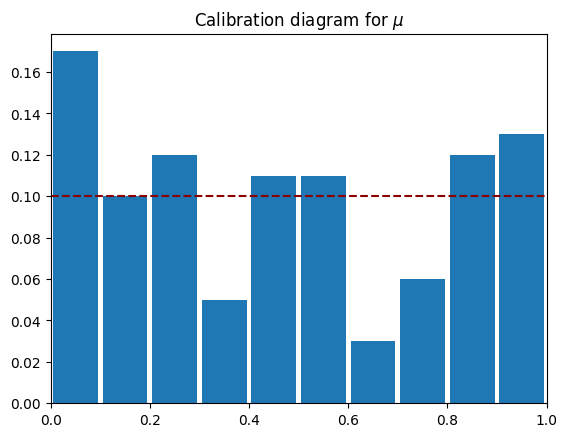
\includegraphics[width=.23\textwidth]{images/sbi_sir/run_1/basic calib mu.png}
    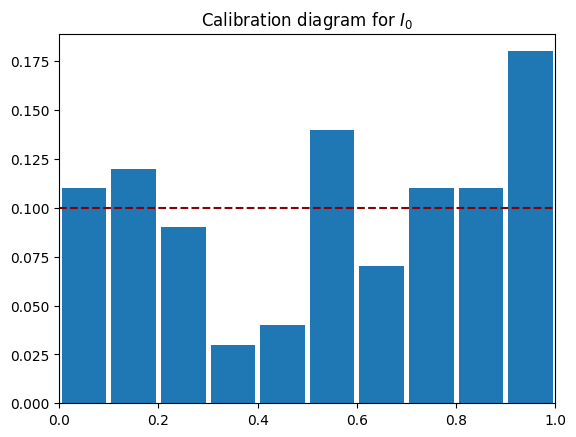
\includegraphics[width=.23\textwidth]{images/sbi_sir/run_1/basic calib I_0.png}
    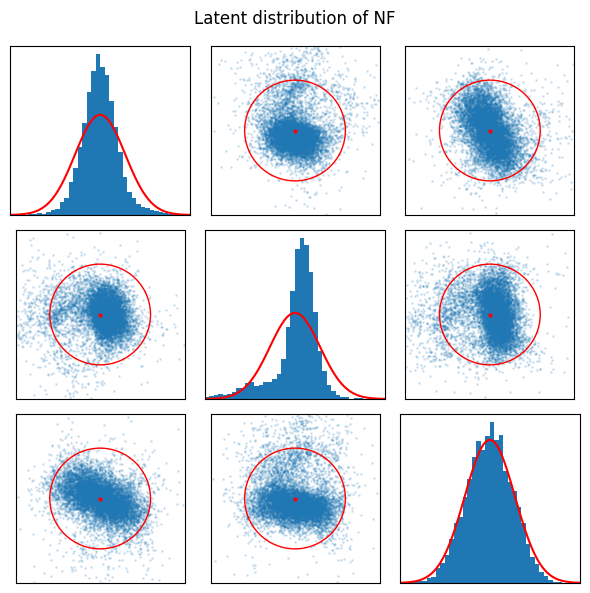
\includegraphics[width=.23\textwidth]{images/sbi_sir/run_1/basic code distribution.png}
    \caption{Calibration diagrams ($\lambda$, $\mu$, and $I_0$, respectively) and code distribution of basic model from the first test.}
\end{subfigure}

\begin{subfigure}{\textwidth}
    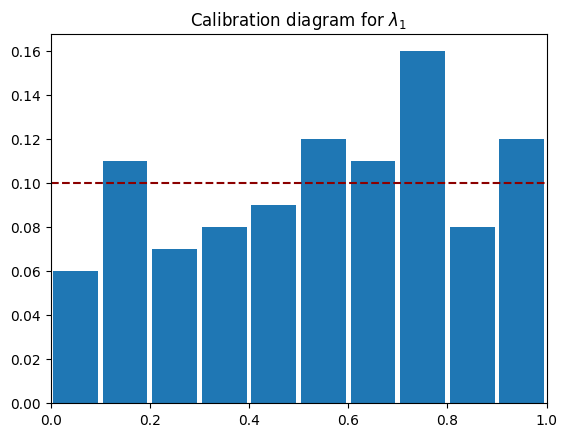
\includegraphics[width=.19\textwidth]{images/sbi_sir/run_1/degen calib lambda1.png}
    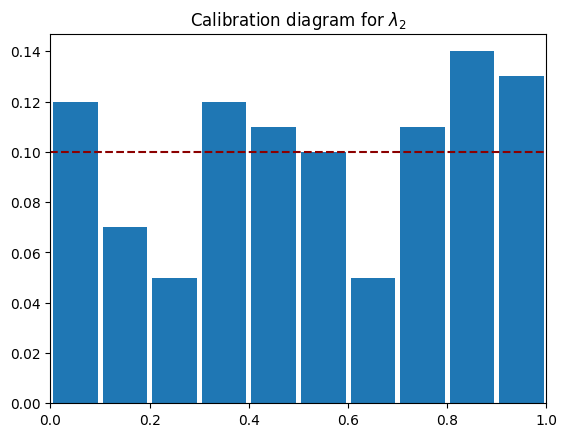
\includegraphics[width=.19\textwidth]{images/sbi_sir/run_1/degen calib lambda2.png}
    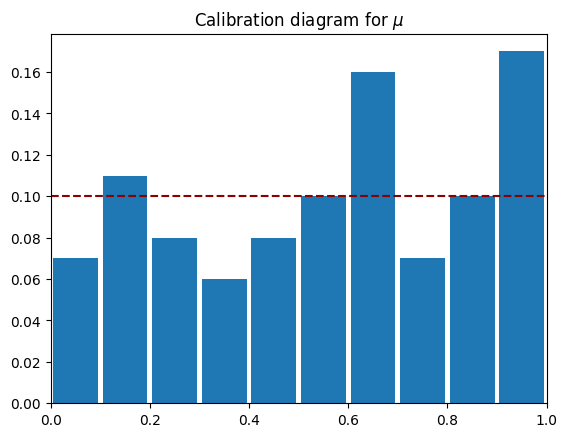
\includegraphics[width=.19\textwidth]{images/sbi_sir/run_1/degen calib mu.png}
    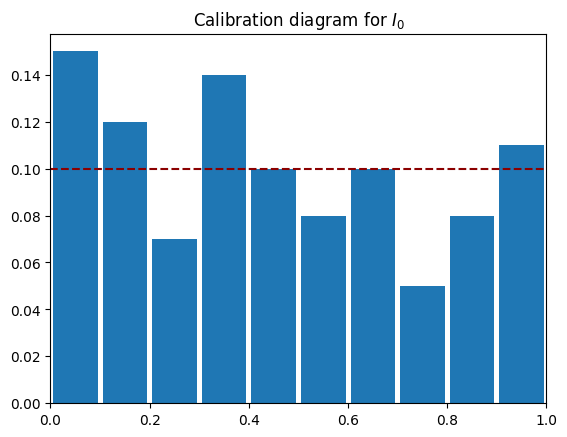
\includegraphics[width=.19\textwidth]{images/sbi_sir/run_1/degen calib I_0.png}
    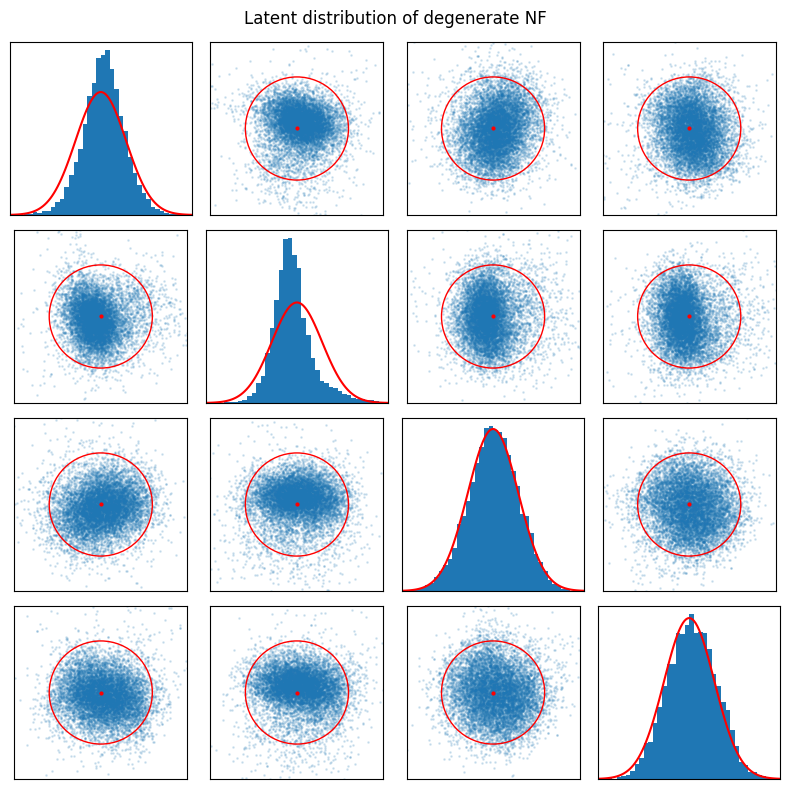
\includegraphics[width=.19\textwidth]{images/sbi_sir/run_1/degen code distribution.png}
    \caption{Calibration diagrams ($\lambda_1$, $\lambda_2$, $\mu$, and $I_0$, respectively) and code distribution of degenerate model from the first test.}
\end{subfigure}
\caption{Evaluation data from the first test.}
\label{fig:sir_run_1}
\end{figure}

\textbf{Experiment 2:} Having fixed \texttt{BijectiveLayer}, we repeated the first test, although we did not have the time to let the models train until convergence. To still get a fair comparison, both models were trained on the exact same hyperparameters, in particular on the same number of epochs (2000 in this case). The results (Figure~\ref{fig:sir_run_2}) were quite surprising:

\begin{figure}[ht]
\centering
\begin{subfigure}{\textwidth}
    \centering
    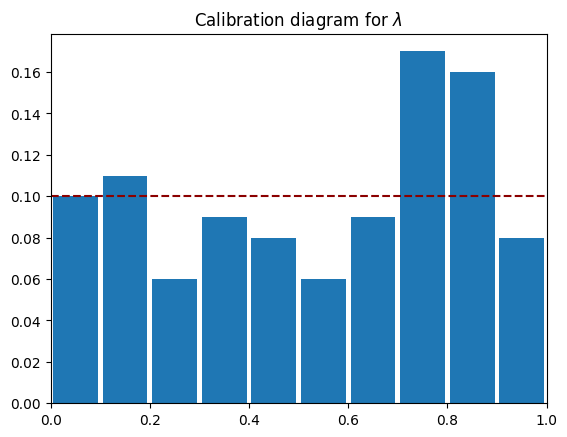
\includegraphics[width=.23\textwidth]{images/sbi_sir/run_2/basic calib lambda.png}
    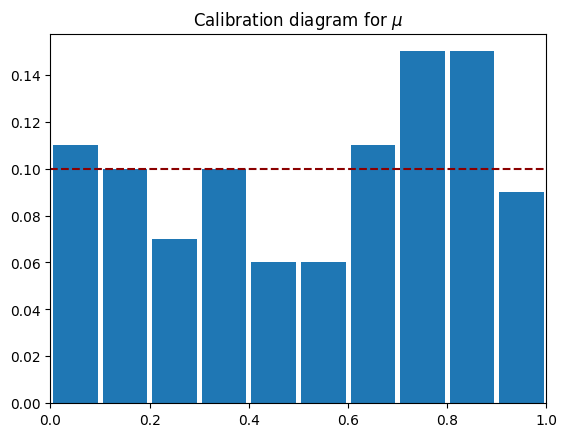
\includegraphics[width=.23\textwidth]{images/sbi_sir/run_2/basic calib mu.png}
    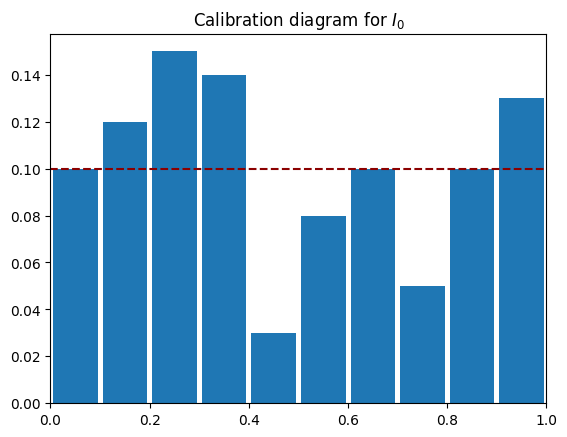
\includegraphics[width=.23\textwidth]{images/sbi_sir/run_2/basic calib I_0.png}
    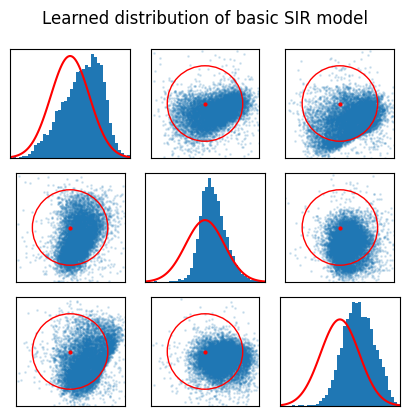
\includegraphics[width=.23\textwidth]{images/sbi_sir/run_2/basic code distribution.png}\\
    \vspace{.5em}
    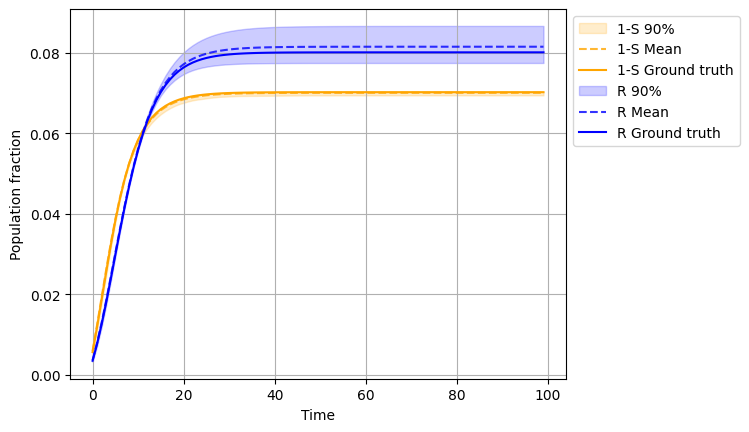
\includegraphics[width=.325\textwidth]{images/sbi_sir/run_2/basic resim 1.png}
    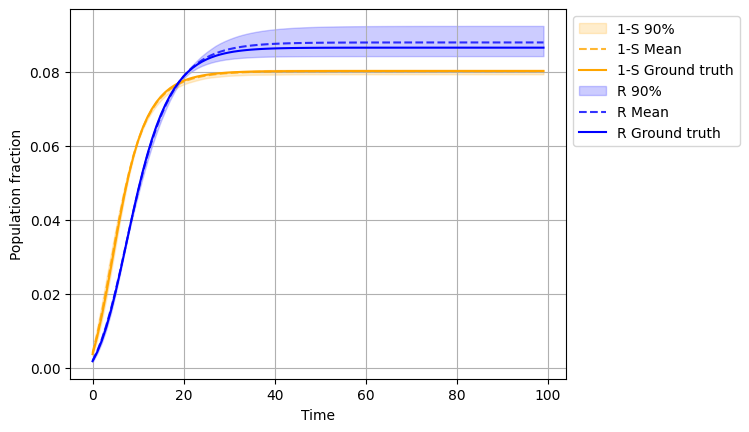
\includegraphics[width=.325\textwidth]{images/sbi_sir/run_2/basic resim 2.png}
    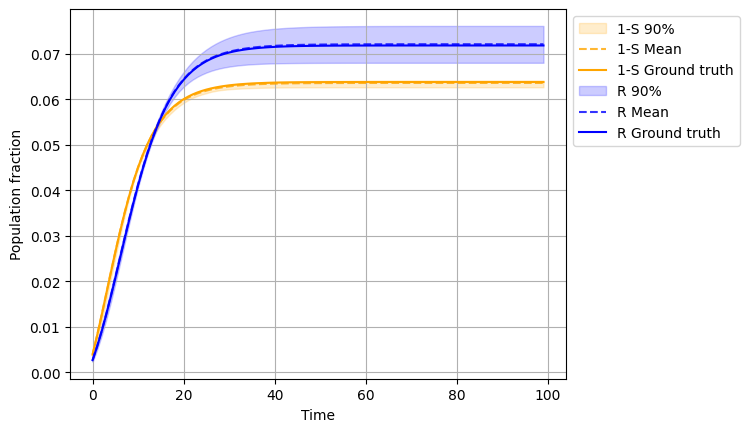
\includegraphics[width=.325\textwidth]{images/sbi_sir/run_2/basic resim 3.png}
    \caption{Calibration diagrams ($\lambda$, $\mu$, and $I_0$, respectively), code distribution and three resimulations of basic model from the second test.}
\end{subfigure}

\begin{subfigure}{\textwidth}
    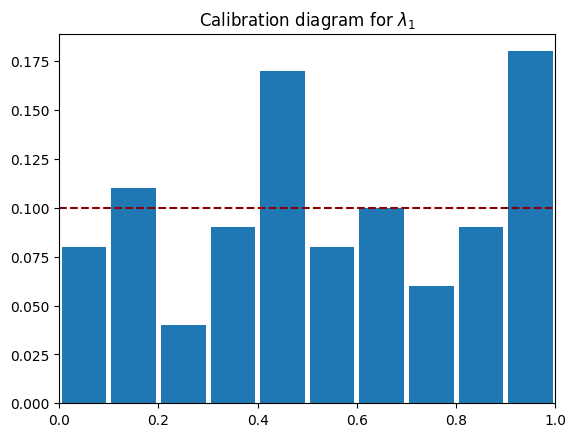
\includegraphics[width=.19\textwidth]{images/sbi_sir/run_2/degen calib lambda1.png}
    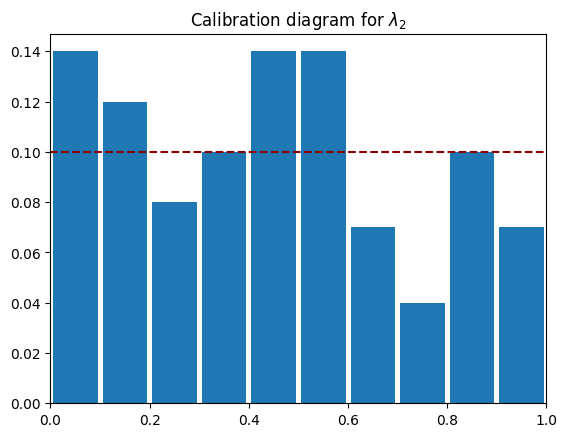
\includegraphics[width=.19\textwidth]{images/sbi_sir/run_2/degen calib lambda2.png}
    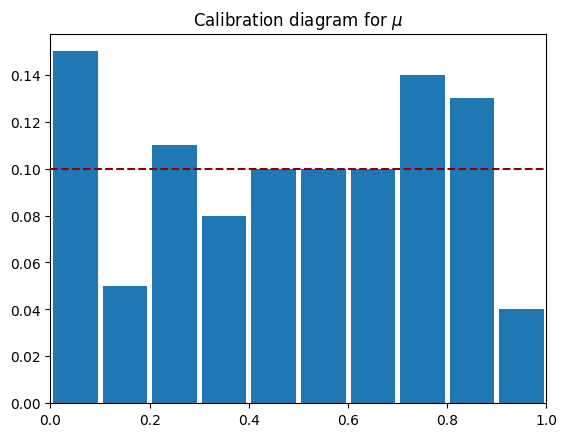
\includegraphics[width=.19\textwidth]{images/sbi_sir/run_2/degen calib mu.png}
    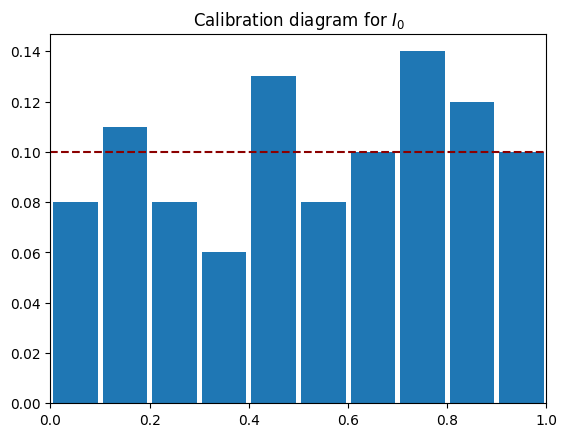
\includegraphics[width=.19\textwidth]{images/sbi_sir/run_2/degen calib I_0.png}
    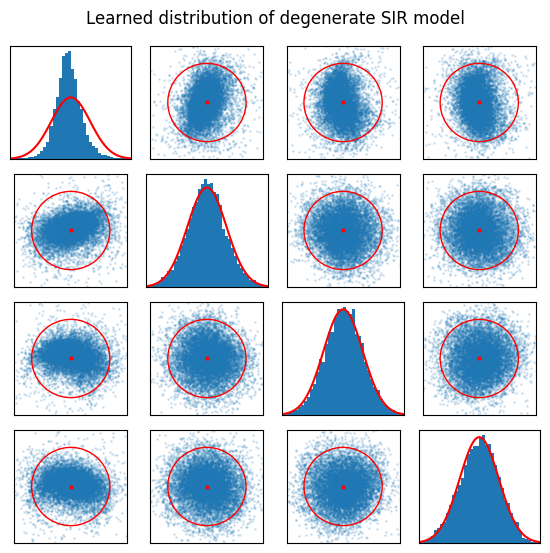
\includegraphics[width=.19\textwidth]{images/sbi_sir/run_2/degen code distribution.png}\\
    \vspace{.5em}
    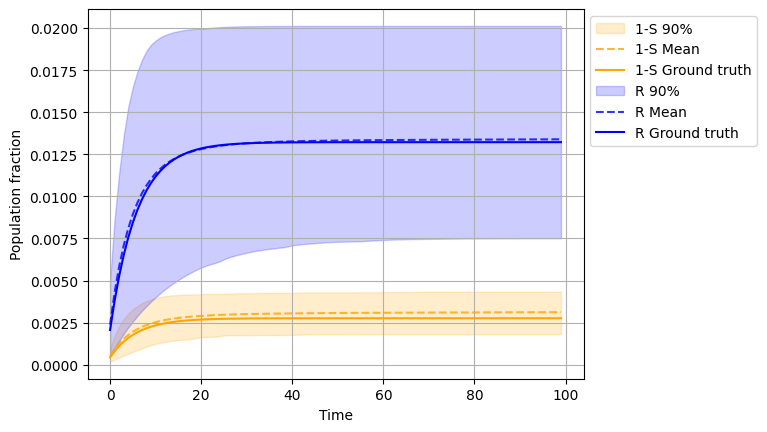
\includegraphics[width=.325\textwidth]{images/sbi_sir/run_2/degen resim 1.png}
    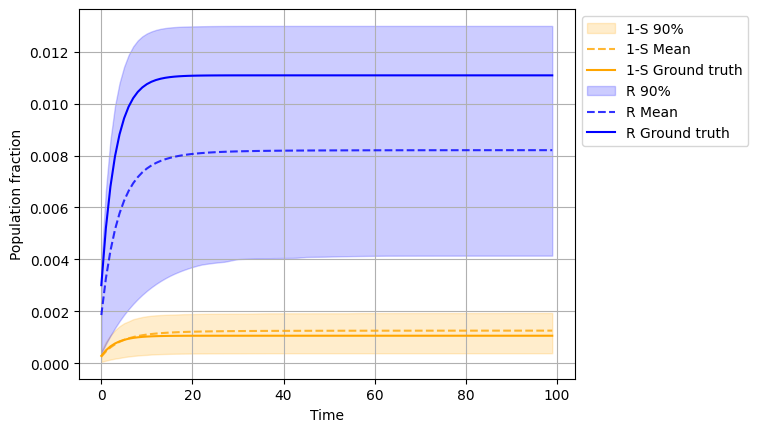
\includegraphics[width=.325\textwidth]{images/sbi_sir/run_2/degen resim 2.png}
    \includegraphics[width=.25\textwidth]{images/sbi_sir/run_2/degen resim 3.png}
    \caption{Calibration diagrams ($\lambda_1$, $\lambda_2$, $\mu$, and $I_0$, respectively), code distribution and three resimulations of degenerate model from the second test.}
\end{subfigure}
\caption{Evaluation data from the second test. }
\label{fig:sir_run_2}
\end{figure}

\begin{itemize}
    \item The code distribution of the basic model looks appalling while that of the degenerate model looks well-behaved except for the first dimension\footnote{Note that the distributions in these plots always have the order $\lambda$, $\mu$, $I_0$ for the basic model and $\lambda_1$, $\lambda_2$, $\mu$, $I_0$ for the degenerate one.}, counter to our expectations. It is also noteworthy that the degenerate model apparently could make better sense of $\lambda_2$ than $\lambda_1$, although this might be down to random chance.
    
    \item The resimulation plots tell a different story: While the ground truth was well within the 90\% confidence interval for both models and all samples, said confidence interval was much narrower for the basic model, insinuating a better understanding of the data.
    
    \item The calibration diagrams all look unpleasant, possibly due to premature training termination. There is no discernible systematic error.
\end{itemize}

In addition to the previously established evaluation data, we also looked at the distribution of sampled parameters for a fixed condition (i.e. the parameters that are used for the resimulation), shown in Figure~\ref{fig:sir_run_2_params}. We were surprised by the spread for the basic model, which is apparently roughly one-dimensional instead of zero-dimensional like we expected, meaning that there is, according to this model, one degree of freedom when fitting parameters to simulation data. In other words, the original ``basic" setup is apparently degenerate. The fact that the resimulation data from this model is so good seems to indicate that this finding indeed stems from the training data itself and not from a poorly trained model. Briefly looking at the sample distribution of the other model, it is clearly higher-dimensional, with the first two dimensions ($\lambda_1$ and $\lambda_2$) forming what looks to be a normal distribution.

\begin{figure}
\centering
\includegraphics[width=.39\textwidth]{images/sbi_sir/run_2/basic param sampling.png}
\hspace{1em}
\includegraphics[width=.52\textwidth]{images/sbi_sir/run_2/degen param sampling.png}
\caption{Parameter sample distribution given fixed condition for basic model (left) and degenerate model (right). All subplots are scaled identically, making them easily comparable.}
\label{fig:sir_run_2_params}
\end{figure}

To be candid, we did not know how to proceed from these findings. It is possible that our initial parameter sampling for the model training was chosen badly, resulting in degeneracy of the supposedly unproblematic training set. Even still, we did not know what to make of the model behaviour, i.e. bad code distribution but near perfect resimulation, since this dichotomy indicates that a standard normalizing flow is able to cope with at least mild levels of degeneracy, rendering this whole experiment pointless. We ultimately decided to lay this test series to rest and instead work with much more straight-forward parameter degeneracy.

\asubsubsection{Simple degeneracy}{Jannis Heising}\label{sec:simple_degen}

\textit{The results are taken from the \href{https://github.com/xiaoxiae/GNNFinal2024/blob/main/notebooks/degen_circle.ipynb}{notebooks/degen\_circle.ipynb} notebook.}

As a simple non-trivial example of degeneracy, we chose the dataset to be points on a perfect circle (i.e. without noise) embedded in 2D euclidean space with an arbitrarily chosen radius of 4. This way, the data is two-dimensional, but its intrinsic dimensionality is only One (the only degree of freedom being the angle in polar coordinates). On this dataset, we trained three different models:

\begin{enumerate}
\item A standard normalizing flow with 20 bijective layers (each of course accompanied by an orthonormal layer). This was chosen as a benchmark to compare to.

\item A SurVAE model with two blocks of 10 bijective layers, separated by a bottleneck (referred to as Bottleneck-SurVAE). The bottleneck was achieved by pairing a \texttt{SliceLayer}, which removes one data entry, with an \texttt{Augment-\linebreak Layer}, which appends a random item. In total, the architecture looked as follows:

\begin{minted}{python}
(BijectiveLayer(2, [200, 200]), OrthonormalLayer(2)) x 10,
SliceLayer(2, 1),
AugmentLayer(1, 2),
(BijectiveLayer(2, [200, 200]), OrthonormalLayer(2)) x 10
\end{minted}

This architecture was driven by the desire to reduce the number of data dimensions via a bottleneck, the main obstacle in this simple scenario being that bijective layers need at least two data entries to function. Furthermore, we wanted to use a model that was similar to the chosen NF model in the number of parameters so as to make the results more comparable.

\item A SurVAE model with 20 bijective layers appended by one \texttt{MaxTheLayer} (referred to as Max-SurVAE). The parameters of \texttt{MaxTheLayer} were set to be learnable. The architecture thus is:

\begin{minted}{python}
(BijectiveLayer(2, [200, 200]), OrthonormalLayer(2)) x 20,
MaxTheLayer(2)
\end{minted}

The design choices for this model were basically the same as for the previous one, just using different functionality of the SurVAE toolkit.
\end{enumerate}

Due to time constraints, our only method of evaluating the results was comparing distribution plots.

For the first and only experiment on this dataset, we performed small preliminary tests to find hyperparameters that worked reasonably well for the NF model and then used the same values for the other two models. The idea behind this setup was to compare the models on the NF's ``home territory" so as to, if anything, skew the results in the baseline's favor. The results are shown in Figure~\ref{fig:circle_results}.

\begin{figure}
\centering
\begin{subfigure}{\textwidth}
    \centering
    \includegraphics[height=.39\textwidth]{images/degen_circle/nf_code_distribution.png}
    \includegraphics[height=.39\textwidth]{images/degen_circle/nf_sample_full.png}
    \includegraphics[height=.39\textwidth]{images/degen_circle/nf_sample_zoomed.png}
    \caption{Code distribution (left), sample distribution (center), and zoomed-in sample distribution (right) from the NF model.}
\end{subfigure}\\
\vspace{1em}
\begin{subfigure}{\textwidth}
    \centering
    \includegraphics[height=.39\textwidth]{images/degen_circle/sv_bottleneck_code_distribution.png}
    \includegraphics[height=.39\textwidth]{images/degen_circle/sv_bottleneck_sample.png}
    \caption{Code distribution (left) and sample distribution (right) from the Bottleneck-SurVAE model.}
\end{subfigure}\\
\vspace{1em}
\begin{subfigure}{\textwidth}
    \centering
    \includegraphics[height=.39\textwidth]{images/degen_circle/sv_max_code_distribution.png}
    \includegraphics[height=.39\textwidth]{images/degen_circle/sv_max_sample.png}
    \caption{Code distribution (left) and sample distribution (right) from the Max-SurVAE model.}
\end{subfigure}
\caption{Results from the first and only experiment on the circle data. The sample distributions show the desired output shape in red.}
\label{fig:circle_results}
\end{figure}

Interestingly, the NF model behaves somewhat similarly to that from Section~\ref{sec:sbi} in that the code distribution looks horrendous but the samples look passable (though not stellar). There is a distinct line of outliers in the samples that highlights a complexity in the dataset which, frankly, we did not think about prior to seeing these results: The support of the dataset (a circle in $\mathbb{R}^2$) is not contractible, in particular it cannot be meaningfully transformed into the contractible support of a normal distribution that is all of $\mathbb{R}^2$.

The Bottleneck-SurVAE model performed abhorrently, although its latent distribution looks better than that of the NF.

The Max-SurVAE model undoubtedly produced the best samples. The line of outliers observed in the NF plot appears here as well, but not nearly as pronounced. The latent distribution looks promising, but definitely not perfect. If we had more time, we would certainly perform more tests with this kind of model.

This experiment shows that SurVAE models have the potential to help learn degenerate datasets, although more testing is needed to form a more concrete conclusion.
\asection{Conclusions and Outlook}{}

\asubsection{Conclusions}{Tomáš Sláma}

The synthetic experiments that we replicated worked as expected and drew the same conclusion as the original paper.
Besides this, the ones we made in addition (conditional) performed poorly due to the lack of symmetries, which reaffirmed the previous conclusion that the \texttt{AbsoluteLayer} works well only for symmetrical data.

Training SpatialMNIST was not successful, most likely due to the combination of not having enough training time and not using transformers instead of the fully connected network for \texttt{BijectiveLayer}.

Since the training parameters were to extensive in the original paper for the image data, we opted to train on the easier MNIST dataset instead.
Sadly, this was not successful either, mostly due to lack of experience with architectures for training image data.

Parameter degeneracy was initially tested on SBI, which did not work and so we opted to try it on a more simple dataset -- a circle.
This eventually looked very promising, but we did not finish this due to time constraints.

\asubsection{Teamwork and Obstacles}{Maria Stickel}
Working as a team was a rewarding and fun experience. Thanks to the fact that we already have been working together on the exercise sheets, setup and organisation was easy and quick. 

The biggest limiting factor of this project was clearly time. When initially choosing the paper, we anticipated three weeks to be enough time to implement and train the models. This has shown to be very optimistic (if not naive) and has lead to worse results by lack of training and possible bugs, which is especially apparent for SpatialMNIST.

\asubsection{Outlook}{Tomáš Sláma}

Further exploring parameter degeneracy would be the next step, since it looked promising in the later tests and could possibly be an improvement over NF.

The image training failed for us but arguably succeeded in the original paper, so determining what was the cause would also be an interesting question.


\newpage

\nocite{*}
\printbibliography[heading=bibintoc,title={Bibliography}]

\end{document}